% Options for packages loaded elsewhere
\PassOptionsToPackage{unicode}{hyperref}
\PassOptionsToPackage{hyphens}{url}
\PassOptionsToPackage{dvipsnames,svgnames,x11names}{xcolor}
%
\documentclass[
  24px,
  letterpaper,
  DIV=11,
  numbers=noendperiod]{scrartcl}

\usepackage{amsmath,amssymb}
\usepackage{lmodern}
\usepackage{iftex}
\ifPDFTeX
  \usepackage[T1]{fontenc}
  \usepackage[utf8]{inputenc}
  \usepackage{textcomp} % provide euro and other symbols
\else % if luatex or xetex
  \usepackage{unicode-math}
  \defaultfontfeatures{Scale=MatchLowercase}
  \defaultfontfeatures[\rmfamily]{Ligatures=TeX,Scale=1}
\fi
% Use upquote if available, for straight quotes in verbatim environments
\IfFileExists{upquote.sty}{\usepackage{upquote}}{}
\IfFileExists{microtype.sty}{% use microtype if available
  \usepackage[]{microtype}
  \UseMicrotypeSet[protrusion]{basicmath} % disable protrusion for tt fonts
}{}
\makeatletter
\@ifundefined{KOMAClassName}{% if non-KOMA class
  \IfFileExists{parskip.sty}{%
    \usepackage{parskip}
  }{% else
    \setlength{\parindent}{0pt}
    \setlength{\parskip}{6pt plus 2pt minus 1pt}}
}{% if KOMA class
  \KOMAoptions{parskip=half}}
\makeatother
\usepackage{xcolor}
\setlength{\emergencystretch}{3em} % prevent overfull lines
\setcounter{secnumdepth}{-\maxdimen} % remove section numbering
% Make \paragraph and \subparagraph free-standing
\ifx\paragraph\undefined\else
  \let\oldparagraph\paragraph
  \renewcommand{\paragraph}[1]{\oldparagraph{#1}\mbox{}}
\fi
\ifx\subparagraph\undefined\else
  \let\oldsubparagraph\subparagraph
  \renewcommand{\subparagraph}[1]{\oldsubparagraph{#1}\mbox{}}
\fi

\usepackage{color}
\usepackage{fancyvrb}
\newcommand{\VerbBar}{|}
\newcommand{\VERB}{\Verb[commandchars=\\\{\}]}
\DefineVerbatimEnvironment{Highlighting}{Verbatim}{commandchars=\\\{\}}
% Add ',fontsize=\small' for more characters per line
\usepackage{framed}
\definecolor{shadecolor}{RGB}{241,243,245}
\newenvironment{Shaded}{\begin{snugshade}}{\end{snugshade}}
\newcommand{\AlertTok}[1]{\textcolor[rgb]{0.68,0.00,0.00}{#1}}
\newcommand{\AnnotationTok}[1]{\textcolor[rgb]{0.37,0.37,0.37}{#1}}
\newcommand{\AttributeTok}[1]{\textcolor[rgb]{0.40,0.45,0.13}{#1}}
\newcommand{\BaseNTok}[1]{\textcolor[rgb]{0.68,0.00,0.00}{#1}}
\newcommand{\BuiltInTok}[1]{\textcolor[rgb]{0.00,0.23,0.31}{#1}}
\newcommand{\CharTok}[1]{\textcolor[rgb]{0.13,0.47,0.30}{#1}}
\newcommand{\CommentTok}[1]{\textcolor[rgb]{0.37,0.37,0.37}{#1}}
\newcommand{\CommentVarTok}[1]{\textcolor[rgb]{0.37,0.37,0.37}{\textit{#1}}}
\newcommand{\ConstantTok}[1]{\textcolor[rgb]{0.56,0.35,0.01}{#1}}
\newcommand{\ControlFlowTok}[1]{\textcolor[rgb]{0.00,0.23,0.31}{#1}}
\newcommand{\DataTypeTok}[1]{\textcolor[rgb]{0.68,0.00,0.00}{#1}}
\newcommand{\DecValTok}[1]{\textcolor[rgb]{0.68,0.00,0.00}{#1}}
\newcommand{\DocumentationTok}[1]{\textcolor[rgb]{0.37,0.37,0.37}{\textit{#1}}}
\newcommand{\ErrorTok}[1]{\textcolor[rgb]{0.68,0.00,0.00}{#1}}
\newcommand{\ExtensionTok}[1]{\textcolor[rgb]{0.00,0.23,0.31}{#1}}
\newcommand{\FloatTok}[1]{\textcolor[rgb]{0.68,0.00,0.00}{#1}}
\newcommand{\FunctionTok}[1]{\textcolor[rgb]{0.28,0.35,0.67}{#1}}
\newcommand{\ImportTok}[1]{\textcolor[rgb]{0.00,0.46,0.62}{#1}}
\newcommand{\InformationTok}[1]{\textcolor[rgb]{0.37,0.37,0.37}{#1}}
\newcommand{\KeywordTok}[1]{\textcolor[rgb]{0.00,0.23,0.31}{#1}}
\newcommand{\NormalTok}[1]{\textcolor[rgb]{0.00,0.23,0.31}{#1}}
\newcommand{\OperatorTok}[1]{\textcolor[rgb]{0.37,0.37,0.37}{#1}}
\newcommand{\OtherTok}[1]{\textcolor[rgb]{0.00,0.23,0.31}{#1}}
\newcommand{\PreprocessorTok}[1]{\textcolor[rgb]{0.68,0.00,0.00}{#1}}
\newcommand{\RegionMarkerTok}[1]{\textcolor[rgb]{0.00,0.23,0.31}{#1}}
\newcommand{\SpecialCharTok}[1]{\textcolor[rgb]{0.37,0.37,0.37}{#1}}
\newcommand{\SpecialStringTok}[1]{\textcolor[rgb]{0.13,0.47,0.30}{#1}}
\newcommand{\StringTok}[1]{\textcolor[rgb]{0.13,0.47,0.30}{#1}}
\newcommand{\VariableTok}[1]{\textcolor[rgb]{0.07,0.07,0.07}{#1}}
\newcommand{\VerbatimStringTok}[1]{\textcolor[rgb]{0.13,0.47,0.30}{#1}}
\newcommand{\WarningTok}[1]{\textcolor[rgb]{0.37,0.37,0.37}{\textit{#1}}}

\providecommand{\tightlist}{%
  \setlength{\itemsep}{0pt}\setlength{\parskip}{0pt}}\usepackage{longtable,booktabs,array}
\usepackage{calc} % for calculating minipage widths
% Correct order of tables after \paragraph or \subparagraph
\usepackage{etoolbox}
\makeatletter
\patchcmd\longtable{\par}{\if@noskipsec\mbox{}\fi\par}{}{}
\makeatother
% Allow footnotes in longtable head/foot
\IfFileExists{footnotehyper.sty}{\usepackage{footnotehyper}}{\usepackage{footnote}}
\makesavenoteenv{longtable}
\usepackage{graphicx}
\makeatletter
\def\maxwidth{\ifdim\Gin@nat@width>\linewidth\linewidth\else\Gin@nat@width\fi}
\def\maxheight{\ifdim\Gin@nat@height>\textheight\textheight\else\Gin@nat@height\fi}
\makeatother
% Scale images if necessary, so that they will not overflow the page
% margins by default, and it is still possible to overwrite the defaults
% using explicit options in \includegraphics[width, height, ...]{}
\setkeys{Gin}{width=\maxwidth,height=\maxheight,keepaspectratio}
% Set default figure placement to htbp
\makeatletter
\def\fps@figure{htbp}
\makeatother

\KOMAoption{captions}{tableheading}
\makeatletter
\makeatother
\makeatletter
\makeatother
\makeatletter
\@ifpackageloaded{caption}{}{\usepackage{caption}}
\AtBeginDocument{%
\ifdefined\contentsname
  \renewcommand*\contentsname{Table of contents}
\else
  \newcommand\contentsname{Table of contents}
\fi
\ifdefined\listfigurename
  \renewcommand*\listfigurename{List of Figures}
\else
  \newcommand\listfigurename{List of Figures}
\fi
\ifdefined\listtablename
  \renewcommand*\listtablename{List of Tables}
\else
  \newcommand\listtablename{List of Tables}
\fi
\ifdefined\figurename
  \renewcommand*\figurename{Figure}
\else
  \newcommand\figurename{Figure}
\fi
\ifdefined\tablename
  \renewcommand*\tablename{Table}
\else
  \newcommand\tablename{Table}
\fi
}
\@ifpackageloaded{float}{}{\usepackage{float}}
\floatstyle{ruled}
\@ifundefined{c@chapter}{\newfloat{codelisting}{h}{lop}}{\newfloat{codelisting}{h}{lop}[chapter]}
\floatname{codelisting}{Listing}
\newcommand*\listoflistings{\listof{codelisting}{List of Listings}}
\makeatother
\makeatletter
\@ifpackageloaded{caption}{}{\usepackage{caption}}
\@ifpackageloaded{subcaption}{}{\usepackage{subcaption}}
\makeatother
\makeatletter
\@ifpackageloaded{tcolorbox}{}{\usepackage[many]{tcolorbox}}
\makeatother
\makeatletter
\@ifundefined{shadecolor}{\definecolor{shadecolor}{rgb}{.97, .97, .97}}
\makeatother
\makeatletter
\makeatother
\ifLuaTeX
  \usepackage{selnolig}  % disable illegal ligatures
\fi
\IfFileExists{bookmark.sty}{\usepackage{bookmark}}{\usepackage{hyperref}}
\IfFileExists{xurl.sty}{\usepackage{xurl}}{} % add URL line breaks if available
\urlstyle{same} % disable monospaced font for URLs
\hypersetup{
  pdftitle={TP metabolites},
  colorlinks=true,
  linkcolor={blue},
  filecolor={Maroon},
  citecolor={Blue},
  urlcolor={Blue},
  pdfcreator={LaTeX via pandoc}}

\title{TP metabolites}
\author{}
\date{}

\begin{document}
\maketitle
\ifdefined\Shaded\renewenvironment{Shaded}{\begin{tcolorbox}[enhanced, interior hidden, borderline west={3pt}{0pt}{shadecolor}, breakable, sharp corners, boxrule=0pt, frame hidden]}{\end{tcolorbox}}\fi

\hypertarget{goals}{%
\section{Goals}\label{goals}}

\begin{itemize}
\item
  Read in \& format sample data
\item
  Match IDs so they can be used with different pathway databases
\item
  Highlight enriched pathways using different methods \& visualisations
\item
  Choose and understand parameters and their impact on the results
\end{itemize}

\hypertarget{input-data}{%
\section{Input data}\label{input-data}}

\texttt{read.table} is a generic function: specify the separator with
\texttt{sep=} , and if there are column names, use
\texttt{header\ =\ T}.

\begin{Shaded}
\begin{Highlighting}[]
\CommentTok{\# Pre{-}filtered metabolite inputs}
\NormalTok{geno.mother.raw }\OtherTok{=} \FunctionTok{read.table}\NormalTok{(}\StringTok{"data/ML\_add\_geno\_mother11\_05\_2023.csv"}\NormalTok{, }\AttributeTok{sep =} \StringTok{";"}\NormalTok{, }\AttributeTok{header =}\NormalTok{ T)}
\NormalTok{gestation.raw }\OtherTok{=} \FunctionTok{read.table}\NormalTok{(}\StringTok{"data/ML\_add\_gestation\_stage\_11\_05\_2023.csv"}\NormalTok{, }\AttributeTok{sep =} \StringTok{";"}\NormalTok{, }\AttributeTok{header =}\NormalTok{ T)}

\CommentTok{\# Annotation database}
\NormalTok{annot.db }\OtherTok{=} \FunctionTok{read.table}\NormalTok{(}\StringTok{"data/ASICS\_annotationID\_2022\_02.csv"}\NormalTok{, }\AttributeTok{sep =} \StringTok{"}\SpecialCharTok{\textbackslash{}t}\StringTok{"}\NormalTok{, }\AttributeTok{header =}\NormalTok{ T)}
\end{Highlighting}
\end{Shaded}

\hypertarget{data-types}{%
\subsection{Data types}\label{data-types}}

The two types of data we will be using are:

\begin{itemize}
\item
  vector
\item
  dataframe
\end{itemize}

Vectors are lists of elements. Vector elements can be named.

\begin{Shaded}
\begin{Highlighting}[]
\NormalTok{v }\OtherTok{=} \FunctionTok{c}\NormalTok{(}\DecValTok{1}\NormalTok{, }\DecValTok{2}\NormalTok{, }\DecValTok{3}\NormalTok{)}
\NormalTok{v}
\end{Highlighting}
\end{Shaded}

\begin{verbatim}
[1] 1 2 3
\end{verbatim}

\begin{Shaded}
\begin{Highlighting}[]
\FunctionTok{names}\NormalTok{(v) }\OtherTok{=} \FunctionTok{c}\NormalTok{(}\StringTok{"a"}\NormalTok{, }\StringTok{"b"}\NormalTok{, }\StringTok{"c"}\NormalTok{)}
\NormalTok{v}
\end{Highlighting}
\end{Shaded}

\begin{verbatim}
a b c 
1 2 3 
\end{verbatim}

Dataframes are tables: they have columns, rows, column names and can
have row names.

\begin{Shaded}
\begin{Highlighting}[]
\NormalTok{df }\OtherTok{=} \FunctionTok{data.frame}\NormalTok{(}\StringTok{"cola"} \OtherTok{=} \FunctionTok{c}\NormalTok{(}\DecValTok{1}\NormalTok{,}\DecValTok{2}\NormalTok{,}\DecValTok{3}\NormalTok{), }\StringTok{"colb"} \OtherTok{=} \FunctionTok{c}\NormalTok{(}\DecValTok{4}\NormalTok{,}\DecValTok{5}\NormalTok{,}\DecValTok{6}\NormalTok{), }\AttributeTok{row.names =} \FunctionTok{c}\NormalTok{(}\StringTok{"row1"}\NormalTok{, }\StringTok{"row2"}\NormalTok{, }\StringTok{"row3"}\NormalTok{))}
\NormalTok{df}
\end{Highlighting}
\end{Shaded}

\begin{verbatim}
     cola colb
row1    1    4
row2    2    5
row3    3    6
\end{verbatim}

\hypertarget{tidyverse}{%
\subsection{Tidyverse}\label{tidyverse}}

Tidyverse is a R package which loads a collection of other packages
designed to work well together for data manipulation. Some packages it
contains are \texttt{tidyr}, \texttt{dplyr}, \texttt{ggplot2}.

The syntax it is based on uses the pipe symbol:
\texttt{\%\textgreater{}\%} , useful for chaining different operations.

\begin{Shaded}
\begin{Highlighting}[]
\NormalTok{df }\SpecialCharTok{\%\textgreater{}\%} \FunctionTok{print}\NormalTok{() }\CommentTok{\# same as print(df)}
\end{Highlighting}
\end{Shaded}

\begin{verbatim}
     cola colb
row1    1    4
row2    2    5
row3    3    6
\end{verbatim}

\begin{center}\rule{0.5\linewidth}{0.5pt}\end{center}

The main operations used in these exercises are:

\begin{itemize}
\item
  \texttt{select()}: for selecting columns by name, can also select
  everything except a column using \texttt{select(-colname)}
\item
  \texttt{filter()}: for filtering rows by a condition, usually based on
  a column
\item
  \texttt{left\_join()}: for joining two dataframes on a common ID
  column
\item
  \texttt{mutate()}: for editing the values of a column
\item
  \texttt{enframe()}: for converting a named vector into a two-column
  dataframe, useful for getting KEGG pathways into the correct format in
  our case
\item
  \texttt{pull()}: converts a dataframe column into a vector, does the
  same thing as \texttt{df\$colname}
\item
  \texttt{rename()}: for renaming column(s)
\item
  \texttt{relocate()}: specify a column name to reorder and place it as
  the first column
\end{itemize}

You can also chain standard functions like \texttt{unique()},
\texttt{na.omit()}.

\begin{center}\rule{0.5\linewidth}{0.5pt}\end{center}

\hypertarget{examples}{%
\subsubsection{Examples}\label{examples}}

Here is an example using the background set:

\begin{Shaded}
\begin{Highlighting}[]
\CommentTok{\# Background set = all measurable metabolites}
\NormalTok{background\_unfiltered }\OtherTok{=} \FunctionTok{read.table}\NormalTok{(}\StringTok{"data/metabolites\_present\_endometre.csv"}\NormalTok{, }\AttributeTok{sep =} \StringTok{";"}\NormalTok{, }\AttributeTok{header =}\NormalTok{ T)}
\FunctionTok{tail}\NormalTok{(background\_unfiltered)}
\end{Highlighting}
\end{Shaded}

\begin{verbatim}
    Metabolite names_asics Match HMDB PubChem KEGG SMILES Comment ChEBI METLIN
132                                        NA                  NA    NA     NA
133                                        NA                  NA    NA     NA
134                                        NA                  NA    NA     NA
135                                        NA                  NA    NA     NA
136                                        NA                  NA    NA     NA
137                                        NA                  NA    NA     NA
     X X.1 X.2 X.3 X.4 X.5 X.6 X.7 X.8 X.9 X.10 X.11 X.12 X.13 X.14 X.15 X.16
132 NA  NA  NA  NA  NA  NA  NA  NA  NA  NA   NA   NA   NA   NA   NA   NA   NA
133 NA  NA  NA  NA  NA  NA  NA  NA  NA  NA   NA   NA   NA   NA   NA   NA   NA
134 NA  NA  NA  NA  NA  NA  NA  NA  NA  NA   NA   NA   NA   NA   NA   NA   NA
135 NA  NA  NA  NA  NA  NA  NA  NA  NA  NA   NA   NA   NA   NA   NA   NA   NA
136 NA  NA  NA  NA  NA  NA  NA  NA  NA  NA   NA   NA   NA   NA   NA   NA   NA
137 NA  NA  NA  NA  NA  NA  NA  NA  NA  NA   NA   NA   NA   NA   NA   NA   NA
\end{verbatim}

\begin{Shaded}
\begin{Highlighting}[]
\NormalTok{background }\OtherTok{=} \FunctionTok{read.table}\NormalTok{(}\StringTok{"data/metabolites\_present\_endometre.csv"}\NormalTok{, }\AttributeTok{sep =} \StringTok{";"}\NormalTok{, }\AttributeTok{header =}\NormalTok{ T) }\SpecialCharTok{\%\textgreater{}\%} 
  \FunctionTok{filter}\NormalTok{(}\SpecialCharTok{!}\FunctionTok{if\_any}\NormalTok{(PubChem, is.na))  }\CommentTok{\# filter out rows that contain NA in column PubChem}
\FunctionTok{tail}\NormalTok{(background)}
\end{Highlighting}
\end{Shaded}

\begin{verbatim}
      Metabolite  names_asics                       Match        HMDB  PubChem
40 Saccaric acid SaccaricAcid               Glucaric acid HMDB0000663    33037
41     Succinate    Succinate               Succinic acid HMDB0000254     1110
42       Taurine      Taurine                     Taurine HMDB0000251     1123
43          TMAO         TMAO      Trimethylamine N-oxide HMDB0000925     1145
44          UDPG         UDPG Uridine diphosphate glucose HMDB0000286 53477679
45 Vanillic acid VanillicAcid               Vanillic acid HMDB0000484     8468
     KEGG
40 C00818
41 C00042
42 C00245
43 C01104
44 C00029
45 C06672
                                                                                                          SMILES
40                                                              [C@H]([C@@H]([C@@H](C(=O)O)O)O)([C@H](C(=O)O)O)O
41                                                                                              C(CC(=O)O)C(=O)O
42                                                                                               C(CS(=O)(=O)O)N
43                                                                                               C[N+](C)(C)[O-]
44 C1=CN(C(=O)NC1=O)[C@@H]2[C@H]([C@H]([C@@H](O2)COP(=O)(O)OP(=O)(O)OC3[C@H]([C@@H]([C@H]([C@@H](O3)CO)O)O)O)O)O
45                                                                                      COC1=C(C=CC(=C1)C(=O)O)O
   Comment ChEBI METLIN  X X.1 X.2 X.3 X.4 X.5 X.6 X.7 X.8 X.9 X.10 X.11 X.12
40       1 16002   5633 NA  NA  NA  NA  NA  NA  NA  NA  NA  NA   NA   NA   NA
41       1 15741    114 NA  NA  NA  NA  NA  NA  NA  NA  NA  NA   NA   NA   NA
42       1 15891     31 NA  NA  NA  NA  NA  NA  NA  NA  NA  NA   NA   NA   NA
43       1 15724   5876 NA  NA  NA  NA  NA  NA  NA  NA  NA  NA   NA   NA   NA
44       1 46229   5278 NA  NA  NA  NA  NA  NA  NA  NA  NA  NA   NA   NA   NA
45       1 30816   5471 NA  NA  NA  NA  NA  NA  NA  NA  NA  NA   NA   NA   NA
   X.13 X.14 X.15 X.16
40   NA   NA   NA   NA
41   NA   NA   NA   NA
42   NA   NA   NA   NA
43   NA   NA   NA   NA
44   NA   NA   NA   NA
45   NA   NA   NA   NA
\end{verbatim}

\begin{center}\rule{0.5\linewidth}{0.5pt}\end{center}

And an example using the raw unfiltered fold changes:

\begin{Shaded}
\begin{Highlighting}[]
\CommentTok{\# Join by metabolite names to get all fold changes with the ID columns (ChEBI, KEGG..)}
\NormalTok{all.fc.file }\OtherTok{=} \FunctionTok{read.table}\NormalTok{(}\StringTok{"data/log2\_FC\_endometrium\_metabolites\_present.csv"}\NormalTok{, }\AttributeTok{sep =} \StringTok{";"}\NormalTok{, }\AttributeTok{header =}\NormalTok{ T) }
\FunctionTok{head}\NormalTok{(all.fc.file)}
\end{Highlighting}
\end{Shaded}

\begin{verbatim}
   metabolites fc_D110vsD90   fc_LWvsMS
1      Lactate   0.20843228  0.07893974
2 Myo-Inositol   0.10919475 -0.20458874
3    L-Glycine   0.04401215 -0.22991271
4      Taurine  -0.07949751 -0.08002337
5    L-Alanine   0.12676021  0.07203598
6     Methanol   0.09152747 -0.21221730
\end{verbatim}

\begin{Shaded}
\begin{Highlighting}[]
\NormalTok{all.fc }\OtherTok{=} \FunctionTok{read.table}\NormalTok{(}\StringTok{"data/log2\_FC\_endometrium\_metabolites\_present.csv"}\NormalTok{, }\AttributeTok{sep =} \StringTok{";"}\NormalTok{, }\AttributeTok{header =}\NormalTok{ T) }\SpecialCharTok{\%\textgreater{}\%} 
  \FunctionTok{left\_join}\NormalTok{(., background }\SpecialCharTok{\%\textgreater{}\%} \FunctionTok{select}\NormalTok{(names\_asics, KEGG), }
            \AttributeTok{by =} \FunctionTok{c}\NormalTok{(}\StringTok{"metabolites"} \OtherTok{=} \StringTok{"names\_asics"}\NormalTok{)) }\SpecialCharTok{\%\textgreater{}\%} 
  \FunctionTok{rename}\NormalTok{(}\StringTok{"gestation"} \OtherTok{=}\NormalTok{ fc\_D110vsD90, }\StringTok{"geno.mother"} \OtherTok{=}\NormalTok{ fc\_LWvsMS)}
\FunctionTok{head}\NormalTok{(all.fc)}
\end{Highlighting}
\end{Shaded}

\begin{verbatim}
   metabolites   gestation geno.mother   KEGG
1      Lactate  0.20843228  0.07893974 C00186
2 Myo-Inositol  0.10919475 -0.20458874   <NA>
3    L-Glycine  0.04401215 -0.22991271 C00037
4      Taurine -0.07949751 -0.08002337 C00245
5    L-Alanine  0.12676021  0.07203598 C00041
6     Methanol  0.09152747 -0.21221730 C00132
\end{verbatim}

\hypertarget{pathway-sets}{%
\section{Pathway sets}\label{pathway-sets}}

Pathway sets are metabolites grouped together by a common function. We
can get pathway sets from KEGG, Reactome, and using metabolic networks.

\hypertarget{kegg}{%
\subsection{KEGG}\label{kegg}}

Using the KEGG API, we can access the database directly inside R. We can
get a list of all pathways for a given organism, and a list of all
compounds per pathway. We can then match them together to get all
metabolites organised into pathways for our organism.

\begin{Shaded}
\begin{Highlighting}[]
\CommentTok{\# Pig KEGG pathways}
\NormalTok{pig.pathways }\OtherTok{=} \FunctionTok{keggList}\NormalTok{(}\StringTok{"pathway"}\NormalTok{, }\StringTok{"ssc"}\NormalTok{) }\SpecialCharTok{\%\textgreater{}\%} 
  \FunctionTok{enframe}\NormalTok{() }\SpecialCharTok{\%\textgreater{}\%} 
  \FunctionTok{mutate}\NormalTok{(}\AttributeTok{name =} \FunctionTok{str\_remove}\NormalTok{(name,}\StringTok{"\^{}ssc"}\NormalTok{), }
         \AttributeTok{value =} \FunctionTok{str\_remove}\NormalTok{(value, }\StringTok{" }\SpecialCharTok{\textbackslash{}\textbackslash{}}\StringTok{{-} Sus scrofa }\SpecialCharTok{\textbackslash{}\textbackslash{}}\StringTok{(pig}\SpecialCharTok{\textbackslash{}\textbackslash{}}\StringTok{)"}\NormalTok{)) }

\CommentTok{\# Compounds per pathways}
\NormalTok{pathway.compounds }\OtherTok{=} \FunctionTok{keggLink}\NormalTok{(}\StringTok{"cpd"}\NormalTok{, }\StringTok{"pathway"}\NormalTok{) }\SpecialCharTok{\%\textgreater{}\%} 
  \FunctionTok{enframe}\NormalTok{() }\SpecialCharTok{\%\textgreater{}\%} 
  \FunctionTok{mutate}\NormalTok{(}\AttributeTok{name =} \FunctionTok{str\_remove}\NormalTok{(name,}\StringTok{"\^{}path:map"}\NormalTok{), }
         \AttributeTok{value =} \FunctionTok{str\_remove}\NormalTok{(value, }\StringTok{"\^{}cpd:"}\NormalTok{))}

\CommentTok{\# Join the pathways we want to use with the compounds, filter out non metabolic pathways}
\NormalTok{kegg.pathways }\OtherTok{=}\NormalTok{ pig.pathways }\SpecialCharTok{\%\textgreater{}\%} 
  \FunctionTok{left\_join}\NormalTok{(., pathway.compounds, }\AttributeTok{by =} \StringTok{"name"}\NormalTok{) }\SpecialCharTok{\%\textgreater{}\%} 
  \FunctionTok{filter}\NormalTok{(}\FunctionTok{str\_starts}\NormalTok{(name, }\StringTok{"01|00"}\NormalTok{), }
\NormalTok{         name }\SpecialCharTok{!=} \StringTok{"01100"}\NormalTok{)}
\end{Highlighting}
\end{Shaded}

\begin{center}\rule{0.5\linewidth}{0.5pt}\end{center}

Other organisms, and a table to convert IDs:

\begin{Shaded}
\begin{Highlighting}[]
\CommentTok{\# Human KEGG pathways}
\NormalTok{human.pathways }\OtherTok{=} \FunctionTok{keggList}\NormalTok{(}\StringTok{"pathway"}\NormalTok{, }\StringTok{"hsa"}\NormalTok{) }\SpecialCharTok{\%\textgreater{}\%} 
  \FunctionTok{enframe}\NormalTok{() }\SpecialCharTok{\%\textgreater{}\%} 
  \FunctionTok{mutate}\NormalTok{(}\AttributeTok{name =} \FunctionTok{str\_remove}\NormalTok{(name,}\StringTok{"\^{}hsa"}\NormalTok{), }
         \AttributeTok{value =} \FunctionTok{str\_remove}\NormalTok{(value, }\StringTok{" }\SpecialCharTok{\textbackslash{}\textbackslash{}}\StringTok{{-} Homo sapiens }\SpecialCharTok{\textbackslash{}\textbackslash{}}\StringTok{(human}\SpecialCharTok{\textbackslash{}\textbackslash{}}\StringTok{)"}\NormalTok{))}

\CommentTok{\# All KEGG pathways}
\NormalTok{all.pathways }\OtherTok{=} \FunctionTok{keggList}\NormalTok{(}\StringTok{"pathway"}\NormalTok{) }\SpecialCharTok{\%\textgreater{}\%} 
  \FunctionTok{enframe}\NormalTok{() }\SpecialCharTok{\%\textgreater{}\%} 
  \FunctionTok{mutate}\NormalTok{(}\AttributeTok{name =} \FunctionTok{str\_remove}\NormalTok{(name,}\StringTok{"\^{}map"}\NormalTok{))}

\CommentTok{\# We can also use the KEGG API to extract the ChEBI IDs for compounds}
\NormalTok{chebi.to.kegg }\OtherTok{=} \FunctionTok{keggConv}\NormalTok{(}\StringTok{"cpd"}\NormalTok{, }\StringTok{"chebi"}\NormalTok{) }\SpecialCharTok{\%\textgreater{}\%} 
  \FunctionTok{enframe}\NormalTok{() }\SpecialCharTok{\%\textgreater{}\%} 
  \FunctionTok{mutate}\NormalTok{(}\AttributeTok{name =} \FunctionTok{str\_remove}\NormalTok{(name,}\StringTok{"\^{}chebi:"}\NormalTok{), }
         \AttributeTok{value =} \FunctionTok{str\_remove}\NormalTok{(value, }\StringTok{"\^{}cpd:"}\NormalTok{)) }\SpecialCharTok{\%\textgreater{}\%}
  \FunctionTok{rename}\NormalTok{(}\StringTok{"ChEBI"} \OtherTok{=} \StringTok{"name"}\NormalTok{, }\StringTok{"KEGG"} \OtherTok{=} \StringTok{"value"}\NormalTok{) }\SpecialCharTok{\%\textgreater{}\%} 
  \FunctionTok{unique}\NormalTok{()}
\end{Highlighting}
\end{Shaded}

\hypertarget{reactome}{%
\subsection{Reactome}\label{reactome}}

Reactome pathways can be downloaded
\href{https://reactome.org/download-data}{here}, in
\texttt{Physical\ Entity\ (PE)\ Identifier\ mapping\ files}
\textgreater{} \texttt{ChEBI\ to\ pathways}.

Reactome has many more pathways than KEGG meaning it is harder to enrich
them. The database contains many pathways not pertaining to metabolism
meaning we would need to filter them (manually?).

\begin{Shaded}
\begin{Highlighting}[]
\CommentTok{\# Create colnames}
\NormalTok{reactome.colnames }\OtherTok{=} \FunctionTok{c}\NormalTok{(}\StringTok{"ChEBI"}\NormalTok{, }\StringTok{"RID"}\NormalTok{, }\StringTok{"URL"}\NormalTok{, }\StringTok{"PathwayName"}\NormalTok{, }\StringTok{"EvidenceCode"}\NormalTok{, }\StringTok{"Species"}\NormalTok{)}

\CommentTok{\# Lowest level pathways}
\NormalTok{reactome.pathways }\OtherTok{=} \FunctionTok{read.table}\NormalTok{(}\StringTok{"data/ChEBI2Reactome\_Pathway.txt"}\NormalTok{, }\AttributeTok{sep =} \StringTok{"}\SpecialCharTok{\textbackslash{}t}\StringTok{"}\NormalTok{,}\AttributeTok{comment.char =} \StringTok{""}\NormalTok{, }\AttributeTok{quote=}\StringTok{""}\NormalTok{, }\AttributeTok{col.names =}\NormalTok{ reactome.colnames) }\SpecialCharTok{\%\textgreater{}\%} 
  \FunctionTok{filter}\NormalTok{(Species }\SpecialCharTok{==} \StringTok{"Sus scrofa"}\NormalTok{) }\SpecialCharTok{\%\textgreater{}\%} \CommentTok{\# Filter only pig pathways}
  \FunctionTok{select}\NormalTok{(ChEBI, PathwayName)}\SpecialCharTok{\%\textgreater{}\%} \CommentTok{\# Select relevant columns}
  \FunctionTok{relocate}\NormalTok{(PathwayName) }\SpecialCharTok{\%\textgreater{}\%} \CommentTok{\# Reorder}
  \FunctionTok{mutate}\NormalTok{(}\AttributeTok{ChEBI =} \FunctionTok{as.character}\NormalTok{(ChEBI)) }\SpecialCharTok{\%\textgreater{}\%} \CommentTok{\# Fix ChEBI IDs being read as numbers}
  \FunctionTok{left\_join}\NormalTok{(., chebi.to.kegg, }\AttributeTok{by =} \StringTok{"ChEBI"}\NormalTok{) }\SpecialCharTok{\%\textgreater{}\%} \CommentTok{\# Join with ChEBI to KEGG df to get KEGG IDs}
  \FunctionTok{select}\NormalTok{(}\SpecialCharTok{{-}}\NormalTok{ChEBI) }\SpecialCharTok{\%\textgreater{}\%} \CommentTok{\# Remove ChEBI column}
  \FunctionTok{na.omit}\NormalTok{()}
\end{Highlighting}
\end{Shaded}

\begin{verbatim}
Warning in left_join(., chebi.to.kegg, by = "ChEBI"): Detected an unexpected many-to-many relationship between `x` and `y`.
i Row 1139 of `x` matches multiple rows in `y`.
i Row 7596 of `y` matches multiple rows in `x`.
i If a many-to-many relationship is expected, set `relationship =
  "many-to-many"` to silence this warning.
\end{verbatim}

\begin{Shaded}
\begin{Highlighting}[]
\CommentTok{\# All level pathways}
\NormalTok{reactome.all.pathways }\OtherTok{=} \FunctionTok{read.table}\NormalTok{(}\StringTok{"data/ChEBI2Reactome\_All\_Levels.txt"}\NormalTok{, }\AttributeTok{sep =} \StringTok{"}\SpecialCharTok{\textbackslash{}t}\StringTok{"}\NormalTok{,}\AttributeTok{comment.char =} \StringTok{""}\NormalTok{, }\AttributeTok{quote=}\StringTok{""}\NormalTok{, }\AttributeTok{col.names =}\NormalTok{ reactome.colnames) }\SpecialCharTok{\%\textgreater{}\%} 
  \FunctionTok{filter}\NormalTok{(Species }\SpecialCharTok{==} \StringTok{"Sus scrofa"}\NormalTok{) }\SpecialCharTok{\%\textgreater{}\%} \CommentTok{\# Filter only pig pathways}
  \FunctionTok{select}\NormalTok{(ChEBI, PathwayName)}\SpecialCharTok{\%\textgreater{}\%} \CommentTok{\# Select relevant columns}
  \FunctionTok{relocate}\NormalTok{(PathwayName) }\SpecialCharTok{\%\textgreater{}\%} \CommentTok{\# Reorder}
  \FunctionTok{mutate}\NormalTok{(}\AttributeTok{ChEBI =} \FunctionTok{as.character}\NormalTok{(ChEBI)) }\SpecialCharTok{\%\textgreater{}\%} \CommentTok{\# Fix ChEBI IDs being read as numbers}
  \FunctionTok{left\_join}\NormalTok{(., chebi.to.kegg, }\AttributeTok{by =} \StringTok{"ChEBI"}\NormalTok{) }\SpecialCharTok{\%\textgreater{}\%} \CommentTok{\# Join with ChEBI to KEGG df to get KEGG IDs}
  \FunctionTok{select}\NormalTok{(}\SpecialCharTok{{-}}\NormalTok{ChEBI) }\SpecialCharTok{\%\textgreater{}\%} \CommentTok{\# Remove ChEBI column}
  \FunctionTok{na.omit}\NormalTok{()}
\end{Highlighting}
\end{Shaded}

\begin{verbatim}
Warning in left_join(., chebi.to.kegg, by = "ChEBI"): Detected an unexpected many-to-many relationship between `x` and `y`.
i Row 2833 of `x` matches multiple rows in `y`.
i Row 13873 of `y` matches multiple rows in `x`.
i If a many-to-many relationship is expected, set `relationship =
  "many-to-many"` to silence this warning.
\end{verbatim}

\hypertarget{metabolic-network}{%
\subsection{Metabolic network}\label{metabolic-network}}

Metabolic networks can be used for various flux-based simulations of
metabolism, but they are also databases of knowledge. We can use
pathway-metabolite information extracted from a network in the same way
as any other pathway set.

\begin{Shaded}
\begin{Highlighting}[]
\CommentTok{\# Metabolites have network{-}specific IDs, this is a mapped ID to KEGG and ChEBI table}
\NormalTok{metab.network.ids }\OtherTok{=} \FunctionTok{read.table}\NormalTok{(}\StringTok{"data/metabolite\_ids.tsv"}\NormalTok{, }\AttributeTok{sep =} \StringTok{"}\SpecialCharTok{\textbackslash{}t}\StringTok{"}\NormalTok{, }\AttributeTok{header =}\NormalTok{ T, }\AttributeTok{quote =} \StringTok{""}\NormalTok{)}
\CommentTok{\# The original file contains nan instead of NA, so replace them:}
\NormalTok{metab.network.ids}\SpecialCharTok{$}\NormalTok{kegg[metab.network.ids}\SpecialCharTok{$}\NormalTok{kegg }\SpecialCharTok{==} \StringTok{"nan"}\NormalTok{] }\OtherTok{=} \ConstantTok{NA}
\NormalTok{metab.network.ids}\SpecialCharTok{$}\NormalTok{chebi[metab.network.ids}\SpecialCharTok{$}\NormalTok{chebi }\SpecialCharTok{==} \StringTok{"nan"}\NormalTok{] }\OtherTok{=} \ConstantTok{NA}

\CommentTok{\# Create a filter to filter out irrelevant pathways (specific to flux simulation)}
\NormalTok{metab.network.filter }\OtherTok{=} \FunctionTok{c}\NormalTok{(}\StringTok{"Artificial reactions"}\NormalTok{, }\StringTok{"Isolated"}\NormalTok{, }\StringTok{"Miscellaneous"}\NormalTok{, }\StringTok{"Pool reactions"}\NormalTok{, }\StringTok{"Exchange/demand reactions"}\NormalTok{, }\StringTok{"Transport reactions"}\NormalTok{)}

\CommentTok{\# Read in the pathway data, map to KEGG and ChEBI, and filter}
\NormalTok{metab.network.pathways }\OtherTok{=} \FunctionTok{read.table}\NormalTok{(}\StringTok{"data/metabolite\_pathways.tsv"}\NormalTok{, }\AttributeTok{sep =} \StringTok{"}\SpecialCharTok{\textbackslash{}t}\StringTok{"}\NormalTok{, }\AttributeTok{header =}\NormalTok{ T) }\SpecialCharTok{\%\textgreater{}\%} 
  \FunctionTok{unique}\NormalTok{() }\SpecialCharTok{\%\textgreater{}\%}
  \FunctionTok{left\_join}\NormalTok{(., metab.network.ids, }\AttributeTok{by =} \StringTok{"metabolite"}\NormalTok{) }\SpecialCharTok{\%\textgreater{}\%} 
  \FunctionTok{filter}\NormalTok{(}\SpecialCharTok{!}\NormalTok{(subsystem }\SpecialCharTok{\%in\%}\NormalTok{ metab.network.filter))}
\end{Highlighting}
\end{Shaded}

\begin{verbatim}
Warning in left_join(., metab.network.ids, by = "metabolite"): Detected an unexpected many-to-many relationship between `x` and `y`.
i Row 226 of `x` matches multiple rows in `y`.
i Row 1 of `y` matches multiple rows in `x`.
i If a many-to-many relationship is expected, set `relationship =
  "many-to-many"` to silence this warning.
\end{verbatim}

\hypertarget{cpdb}{%
\subsection{CPDB}\label{cpdb}}

ConsensusPathDB is a compiled database of various pathway sets,
including Reactome, KEGG, BioCyc and others. We are using it as an
example of a very large pathway set database.

The database can be downloaded from \url{http://cpdb.molgen.mpg.de/}:
\textgreater{} ``Biological pathways (as defined by source databases)
with their metabolites identified with KEGG / ChEBI / Pubchem-compound
accession numbers''

\begin{Shaded}
\begin{Highlighting}[]
\NormalTok{cpdb }\OtherTok{=} \FunctionTok{read.table}\NormalTok{(}\StringTok{"data/CPDB\_pathways\_metabolites.tab"}\NormalTok{, }\AttributeTok{sep =} \StringTok{"}\SpecialCharTok{\textbackslash{}t}\StringTok{"}\NormalTok{, }\AttributeTok{comment.char =} \StringTok{""}\NormalTok{, }\AttributeTok{header =}\NormalTok{ T) }\SpecialCharTok{\%\textgreater{}\%}
  \FunctionTok{cSplit}\NormalTok{(}\StringTok{"metabolites"}\NormalTok{, }\StringTok{","}\NormalTok{,}\AttributeTok{direction =} \StringTok{"long"}\NormalTok{) }\SpecialCharTok{\%\textgreater{}\%} 
  \FunctionTok{unique}\NormalTok{() }\SpecialCharTok{\%\textgreater{}\%} 
  \FunctionTok{mutate}\NormalTok{(}\AttributeTok{metabolites =} \FunctionTok{str\_remove}\NormalTok{(metabolites, }\StringTok{"\^{}kegg:"}\NormalTok{),}
         \AttributeTok{pathway =} \FunctionTok{str\_remove}\NormalTok{(pathway, }\StringTok{" {-} Homo sapiens }\SpecialCharTok{\textbackslash{}\textbackslash{}}\StringTok{(human}\SpecialCharTok{\textbackslash{}\textbackslash{}}\StringTok{)$"}\NormalTok{))}
\end{Highlighting}
\end{Shaded}

\begin{verbatim}
Warning in type.convert.default(unlist(x, use.names = FALSE)): 'as.is' should
be specified by the caller; using TRUE
\end{verbatim}

\hypertarget{ora}{%
\section{ORA}\label{ora}}

Cluster profiler is normally used with gene enrichment and therefore has
direct access to gene pathway set databases. For metabolites we will
need to specify a custom pathway set.

Important parameters:

\begin{itemize}
\item
  \texttt{gene}: a vector of IDs = pre-filtered metabolite IDs
\item
  \texttt{TERM2GENE}: a two column data.frame of pathway names and
  metabolite IDs = custom pathway set
\item
  \texttt{universe}: a vector of IDs = background dataset
\item
  \texttt{pAdjustMethod}: ``BH'' by default, one of ``holm'',
  ``hochberg'', ``hommel'', ``bonferroni'', ``BH'', ``BY'', ``fdr'',
  ``none''
\item
  \texttt{pvalueCutoff} and \texttt{qvalueCutoff}: default = 0.05 and
  0.2 respectively
\end{itemize}

\hypertarget{basic-ora}{%
\subsection{Basic ORA}\label{basic-ora}}

We will use the KEGG IDs in the input data and perform ORA using the
KEGG pathway sets. By default, the background set is the entire list of
metabolites in the pathway set.

\hypertarget{geno-mother-dataset}{%
\subsubsection{Geno mother dataset}\label{geno-mother-dataset}}

\begin{Shaded}
\begin{Highlighting}[]
\NormalTok{ora.geno.mother.kegg }\OtherTok{=} \FunctionTok{enricher}\NormalTok{(geno.mother.raw}\SpecialCharTok{$}\NormalTok{KEGG , }\AttributeTok{TERM2GENE =}\NormalTok{ kegg.pathways }\SpecialCharTok{\%\textgreater{}\%} \FunctionTok{select}\NormalTok{(}\SpecialCharTok{{-}}\NormalTok{name))}
\FunctionTok{dotplot}\NormalTok{(ora.geno.mother.kegg)}
\end{Highlighting}
\end{Shaded}

\begin{figure}[H]

{\centering 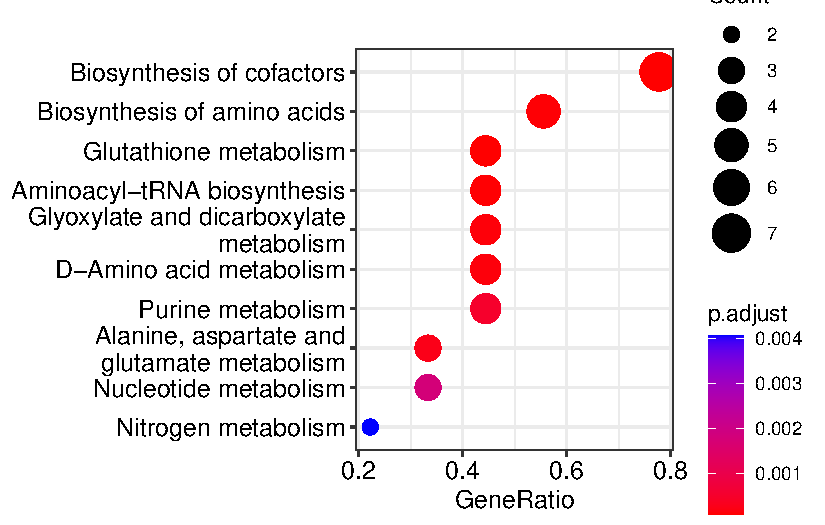
\includegraphics{index_files/figure-pdf/unnamed-chunk-14-1.pdf}

}

\end{figure}

\begin{center}\rule{0.5\linewidth}{0.5pt}\end{center}

\hypertarget{gestation-data-set}{%
\subsubsection{Gestation data set}\label{gestation-data-set}}

\begin{Shaded}
\begin{Highlighting}[]
\NormalTok{ora.gestation.kegg }\OtherTok{=} \FunctionTok{enricher}\NormalTok{(gestation.raw}\SpecialCharTok{$}\NormalTok{KEGG, }\AttributeTok{TERM2GENE =}\NormalTok{ kegg.pathways }\SpecialCharTok{\%\textgreater{}\%} \FunctionTok{select}\NormalTok{(}\SpecialCharTok{{-}}\NormalTok{name))}
\FunctionTok{dotplot}\NormalTok{(ora.gestation.kegg)}
\end{Highlighting}
\end{Shaded}

\begin{figure}[H]

{\centering 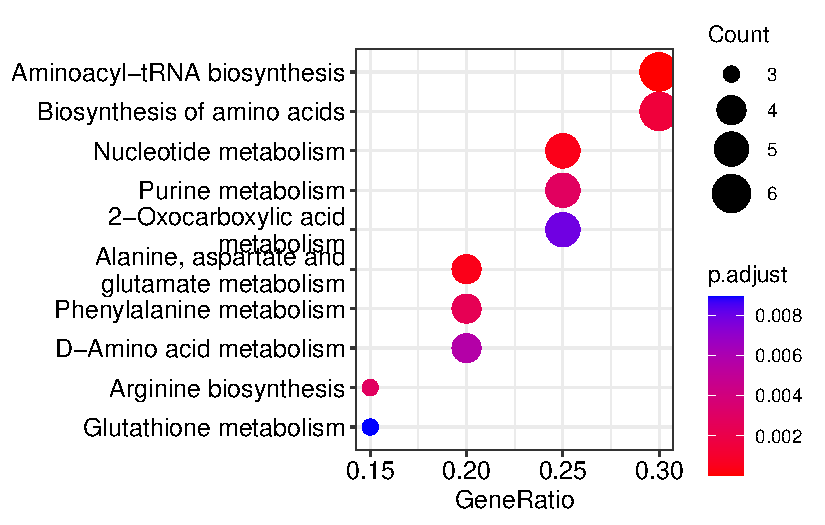
\includegraphics{index_files/figure-pdf/unnamed-chunk-15-1.pdf}

}

\end{figure}

\hypertarget{varying-background-set}{%
\subsection{Varying background set}\label{varying-background-set}}

Changing the background set will completely change the resulting pathway
significance, usually reducing the number of significant pathways. In
metabolomics, we should use the set of measurable metabolites during the
experiment. Depending on if it was targeted or untargeted, this set may
be larger or smaller.

\begin{Shaded}
\begin{Highlighting}[]
\CommentTok{\# Using the background set}
\NormalTok{ora.geno.mother.kegg }\OtherTok{=} \FunctionTok{enricher}\NormalTok{(geno.mother.raw}\SpecialCharTok{$}\NormalTok{KEGG , }\AttributeTok{TERM2GENE =}\NormalTok{ kegg.pathways }\SpecialCharTok{\%\textgreater{}\%} \FunctionTok{select}\NormalTok{(}\SpecialCharTok{{-}}\NormalTok{name),}
                                \AttributeTok{universe =}\NormalTok{ background }\SpecialCharTok{\%\textgreater{}\%} \FunctionTok{pull}\NormalTok{(KEGG))}
\FunctionTok{dotplot}\NormalTok{(ora.geno.mother.kegg)}
\end{Highlighting}
\end{Shaded}

\begin{figure}[H]

{\centering 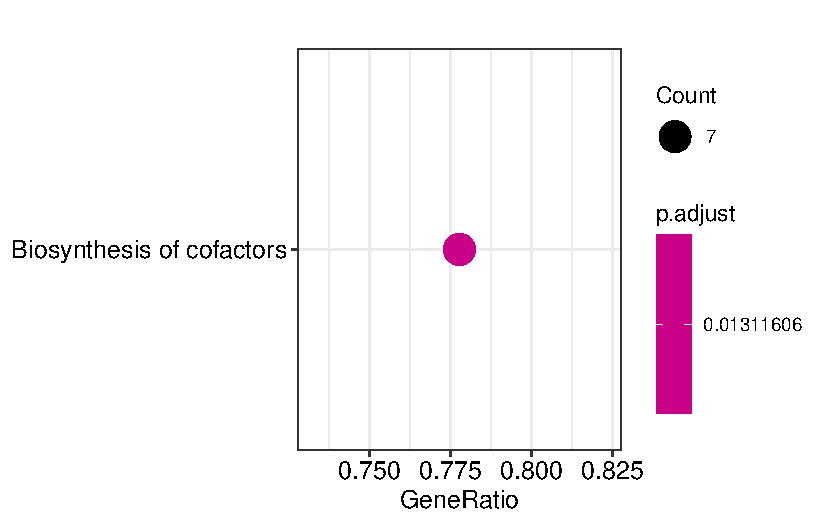
\includegraphics{index_files/figure-pdf/unnamed-chunk-16-1.pdf}

}

\end{figure}

\begin{center}\rule{0.5\linewidth}{0.5pt}\end{center}

Using a restrictive background set means that we get fewer enriched
pathways. However, biologically and statistically we must use a
background set reflective of what could have been measured.

\begin{figure}

{\centering 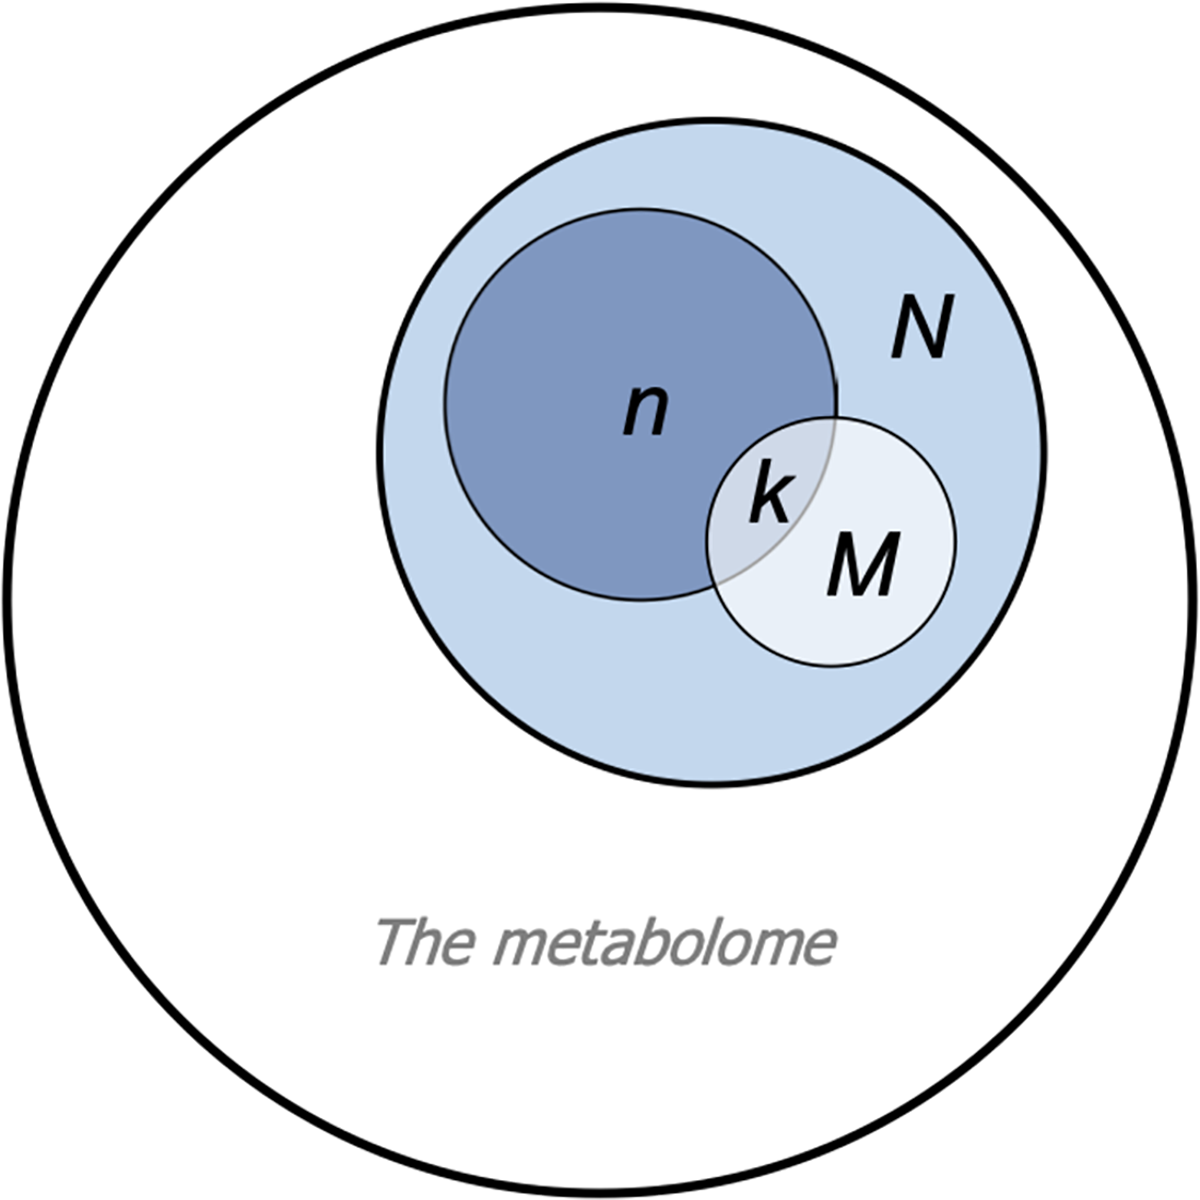
\includegraphics[width=3.46875in,height=\textheight]{images/ora.PNG}

}

\end{figure}

N = background set

n = input metabolites of interest

M = metabolites in pathway being tested against

k = overlap between n and M

\begin{center}\rule{0.5\linewidth}{0.5pt}\end{center}

\hypertarget{using-the-annotation-set-as-an-example}{%
\subsubsection{Using the annotation set as an
example}\label{using-the-annotation-set-as-an-example}}

\begin{Shaded}
\begin{Highlighting}[]
\NormalTok{ora.geno.mother.kegg }\OtherTok{=} \FunctionTok{enricher}\NormalTok{(geno.mother.raw}\SpecialCharTok{$}\NormalTok{KEGG , }\AttributeTok{TERM2GENE =}\NormalTok{ kegg.pathways }\SpecialCharTok{\%\textgreater{}\%} \FunctionTok{select}\NormalTok{(}\SpecialCharTok{{-}}\NormalTok{name),}
                                \AttributeTok{universe =}\NormalTok{ annot.db }\SpecialCharTok{\%\textgreater{}\%} \FunctionTok{pull}\NormalTok{(KEGG))}
\FunctionTok{dotplot}\NormalTok{(ora.geno.mother.kegg)}
\end{Highlighting}
\end{Shaded}

\begin{figure}[H]

{\centering 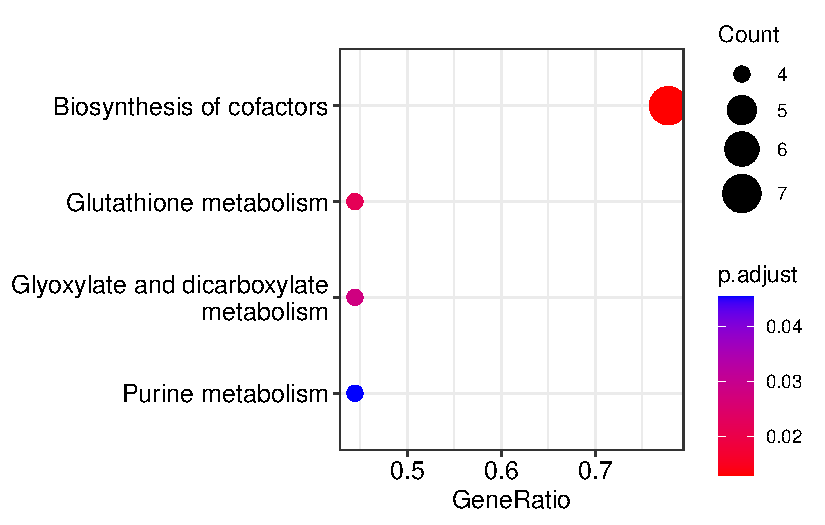
\includegraphics{index_files/figure-pdf/unnamed-chunk-17-1.pdf}

}

\end{figure}

\hypertarget{varying-pathway-database}{%
\subsection{Varying pathway database}\label{varying-pathway-database}}

Instead of KEGG pathways, we can use the metabolic network pathways or
Reactome pathways.

\hypertarget{metabolic-network-1}{%
\subsubsection{Metabolic network}\label{metabolic-network-1}}

\begin{Shaded}
\begin{Highlighting}[]
\NormalTok{ora.geno.mother.metnet }\OtherTok{=} \FunctionTok{enricher}\NormalTok{(geno.mother.raw}\SpecialCharTok{$}\NormalTok{KEGG , }\AttributeTok{TERM2GENE =}\NormalTok{ metab.network.pathways }\SpecialCharTok{\%\textgreater{}\%} 
                                    \FunctionTok{select}\NormalTok{(subsystem, kegg) }\SpecialCharTok{\%\textgreater{}\%} \FunctionTok{na.omit}\NormalTok{(), }
                                  \AttributeTok{universe =}\NormalTok{ annot.db }\SpecialCharTok{\%\textgreater{}\%} \FunctionTok{pull}\NormalTok{(KEGG))}
\FunctionTok{dotplot}\NormalTok{(ora.geno.mother.metnet)}
\end{Highlighting}
\end{Shaded}

\begin{figure}[H]

{\centering 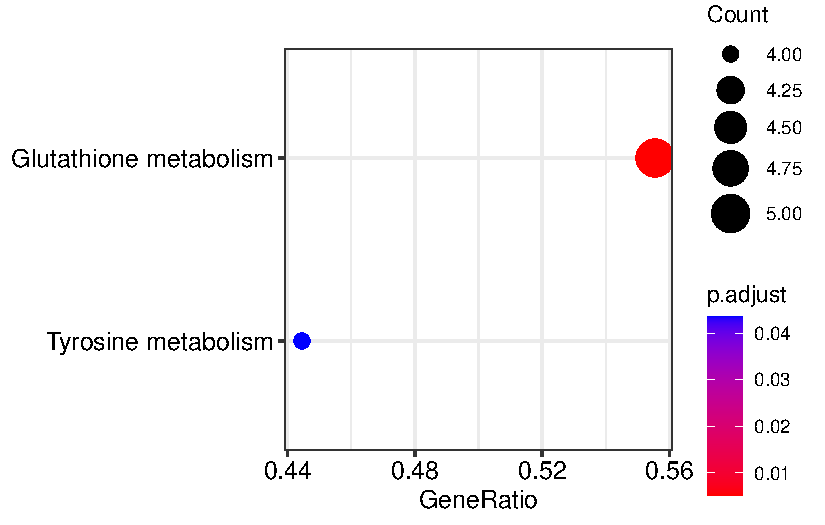
\includegraphics{index_files/figure-pdf/unnamed-chunk-18-1.pdf}

}

\end{figure}

\begin{center}\rule{0.5\linewidth}{0.5pt}\end{center}

Using the second larger dataset, it is harder to gain significantly
enriched pathways. Using the metabolic network pathways, we are unable
to get any enriched pathways even with no p-value cutoff. Only by
removing the background set are we able to get enrichment.

\begin{Shaded}
\begin{Highlighting}[]
\NormalTok{ora.gestation.metnet }\OtherTok{=} \FunctionTok{enricher}\NormalTok{(gestation.raw}\SpecialCharTok{$}\NormalTok{KEGG , }\AttributeTok{TERM2GENE =}\NormalTok{ metab.network.pathways }\SpecialCharTok{\%\textgreater{}\%} \FunctionTok{select}\NormalTok{(subsystem, kegg) }\SpecialCharTok{\%\textgreater{}\%} \FunctionTok{na.omit}\NormalTok{())}
\FunctionTok{dotplot}\NormalTok{(ora.gestation.metnet)}
\end{Highlighting}
\end{Shaded}

\begin{figure}[H]

{\centering 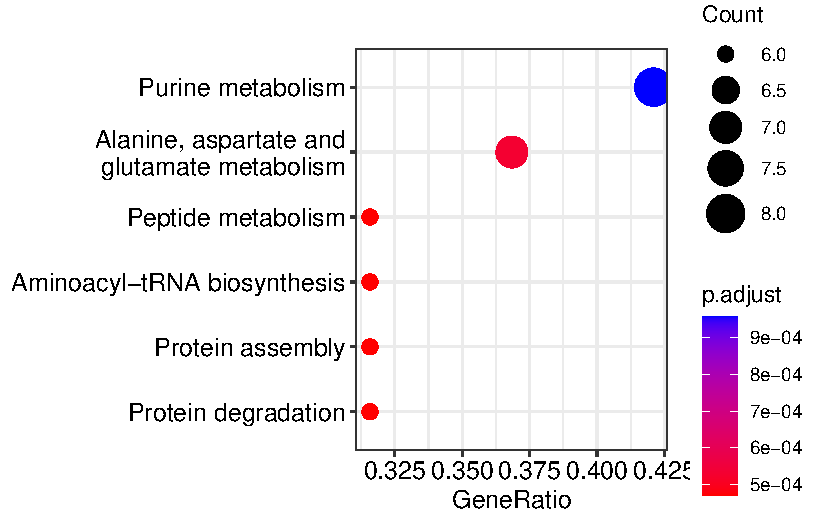
\includegraphics{index_files/figure-pdf/unnamed-chunk-19-1.pdf}

}

\end{figure}

\begin{center}\rule{0.5\linewidth}{0.5pt}\end{center}

\hypertarget{reactome-1}{%
\subsubsection{Reactome}\label{reactome-1}}

Reactome is a larger pathway set, meaning we need to use no background
set (!) to get significant pathways.

\begin{Shaded}
\begin{Highlighting}[]
\NormalTok{ora.gestation.reactome }\OtherTok{=} \FunctionTok{enricher}\NormalTok{(gestation.raw}\SpecialCharTok{$}\NormalTok{KEGG , }\AttributeTok{TERM2GENE =}\NormalTok{ reactome.pathways)}
\FunctionTok{dotplot}\NormalTok{(ora.gestation.reactome)}
\end{Highlighting}
\end{Shaded}

\begin{figure}[H]

{\centering 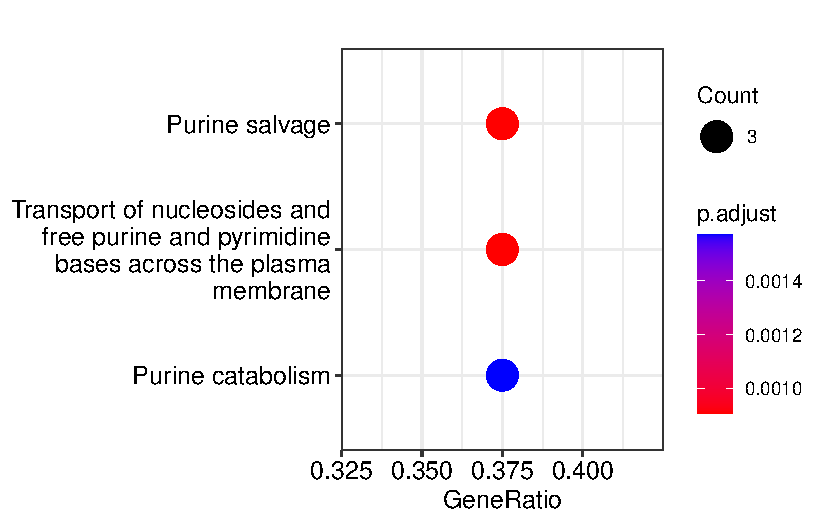
\includegraphics{index_files/figure-pdf/unnamed-chunk-20-1.pdf}

}

\end{figure}

\begin{center}\rule{0.5\linewidth}{0.5pt}\end{center}

As you can see, even though the p-values are low, having only one
metabolite enrich each pathway is not necessarily relevant.

\begin{Shaded}
\begin{Highlighting}[]
\NormalTok{ora.geno.mother.reactome }\OtherTok{=} \FunctionTok{enricher}\NormalTok{(geno.mother.raw}\SpecialCharTok{$}\NormalTok{KEGG , }\AttributeTok{TERM2GENE =}\NormalTok{ reactome.pathways,}
                                    \AttributeTok{pvalueCutoff =} \FloatTok{0.1}\NormalTok{)}
\FunctionTok{dotplot}\NormalTok{(ora.geno.mother.reactome)}
\end{Highlighting}
\end{Shaded}

\begin{figure}[H]

{\centering 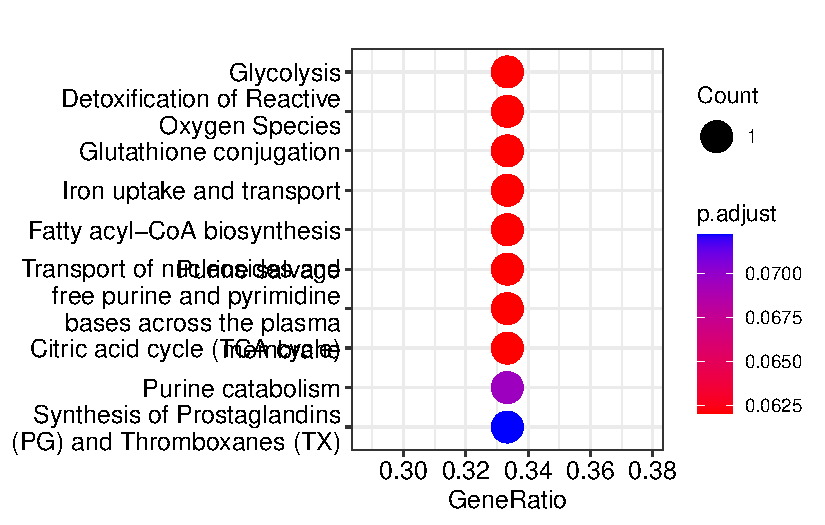
\includegraphics{index_files/figure-pdf/unnamed-chunk-21-1.pdf}

}

\end{figure}

\begin{center}\rule{0.5\linewidth}{0.5pt}\end{center}

\hypertarget{cpdb-1}{%
\subsubsection{CPDB}\label{cpdb-1}}

Here is an example of using a non filtered pathway set database. We
obtain many non-metabolic pathways that are enriched but are meaningless
in terms of our input data.

\begin{Shaded}
\begin{Highlighting}[]
\NormalTok{ora.gestation.cpdb }\OtherTok{=} \FunctionTok{enricher}\NormalTok{(gestation.raw}\SpecialCharTok{$}\NormalTok{KEGG, }
                              \AttributeTok{TERM2GENE =}\NormalTok{ cpdb }\SpecialCharTok{\%\textgreater{}\%} \FunctionTok{filter}\NormalTok{(source }\SpecialCharTok{==} \StringTok{"Reactome"}\NormalTok{) }\SpecialCharTok{\%\textgreater{}\%} \FunctionTok{select}\NormalTok{(}\SpecialCharTok{{-}}\NormalTok{source))}
\FunctionTok{dotplot}\NormalTok{(ora.gestation.cpdb)}
\end{Highlighting}
\end{Shaded}

\begin{figure}[H]

{\centering 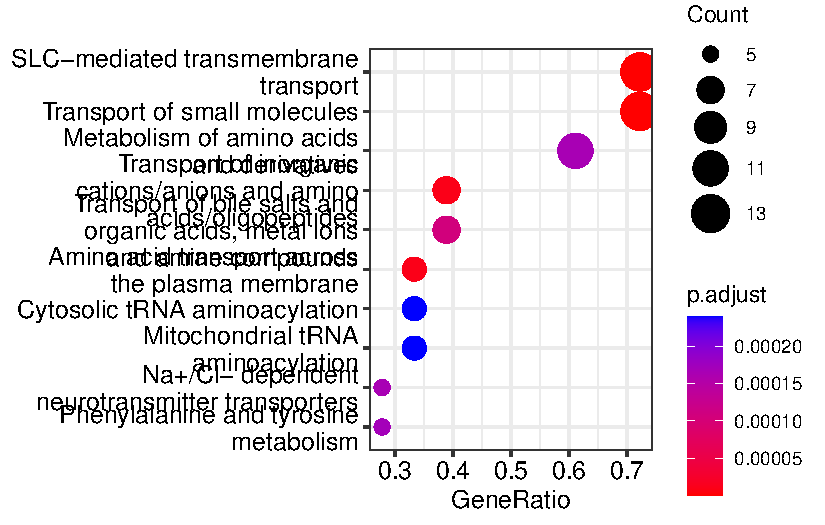
\includegraphics{index_files/figure-pdf/unnamed-chunk-22-1.pdf}

}

\end{figure}

\hypertarget{varying-significant-metabolites}{%
\subsection{Varying significant
metabolites}\label{varying-significant-metabolites}}

The initial filtering of measured metabolites can also change the
resulting enrichment. Here we can use a strict filtering of the fold
changes in the initial dataset. Since it is stricter, we can't use a
background set in this example since we wouldn't get any results.

\begin{Shaded}
\begin{Highlighting}[]
\NormalTok{gestation.filtered }\OtherTok{=}\NormalTok{ all.fc }\SpecialCharTok{\%\textgreater{}\%} \FunctionTok{select}\NormalTok{(}\SpecialCharTok{{-}}\NormalTok{geno.mother) }\SpecialCharTok{\%\textgreater{}\%}
  \FunctionTok{filter}\NormalTok{(}\FunctionTok{abs}\NormalTok{(gestation) }\SpecialCharTok{\textgreater{}} \DecValTok{1}\NormalTok{)}
\NormalTok{ora.gestation.filtered.kegg }\OtherTok{=} \FunctionTok{enricher}\NormalTok{(gestation.filtered}\SpecialCharTok{$}\NormalTok{KEGG , }\AttributeTok{TERM2GENE =}\NormalTok{ kegg.pathways }\SpecialCharTok{\%\textgreater{}\%} \FunctionTok{select}\NormalTok{(}\SpecialCharTok{{-}}\NormalTok{name))}
\FunctionTok{dotplot}\NormalTok{(ora.gestation.filtered.kegg)}
\end{Highlighting}
\end{Shaded}

\begin{figure}[H]

{\centering 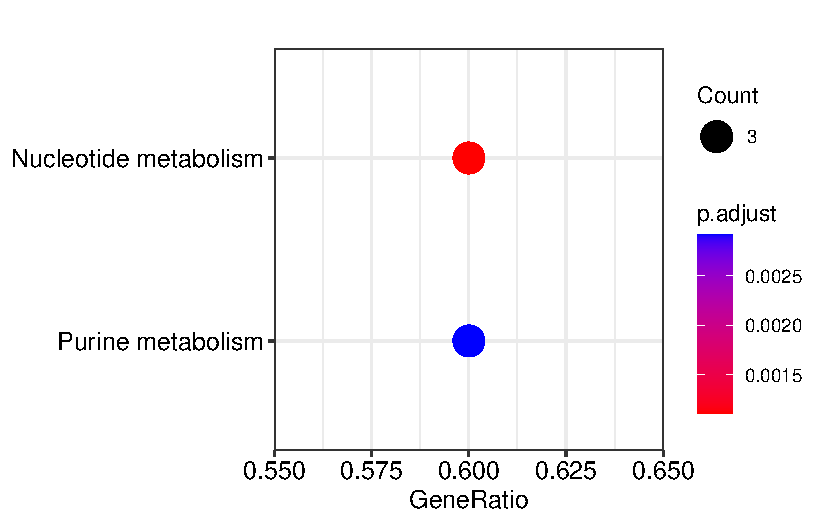
\includegraphics{index_files/figure-pdf/unnamed-chunk-23-1.pdf}

}

\end{figure}

\begin{center}\rule{0.5\linewidth}{0.5pt}\end{center}

We can also use a more relaxed threshold on this dataset's fold changes,
again without a background set for illustration purposes.

\begin{Shaded}
\begin{Highlighting}[]
\NormalTok{gestation.filtered }\OtherTok{=}\NormalTok{ all.fc }\SpecialCharTok{\%\textgreater{}\%} \FunctionTok{select}\NormalTok{(}\SpecialCharTok{{-}}\NormalTok{geno.mother) }\SpecialCharTok{\%\textgreater{}\%}
  \FunctionTok{filter}\NormalTok{(}\FunctionTok{abs}\NormalTok{(gestation) }\SpecialCharTok{\textgreater{}} \FloatTok{0.1}\NormalTok{)}
\NormalTok{ora.gestation.filtered.kegg }\OtherTok{=} \FunctionTok{enricher}\NormalTok{(gestation.filtered}\SpecialCharTok{$}\NormalTok{KEGG , }\AttributeTok{TERM2GENE =}\NormalTok{ kegg.pathways }\SpecialCharTok{\%\textgreater{}\%} \FunctionTok{select}\NormalTok{(}\SpecialCharTok{{-}}\NormalTok{name))}
\FunctionTok{dotplot}\NormalTok{(ora.gestation.filtered.kegg)}
\end{Highlighting}
\end{Shaded}

\begin{figure}[H]

{\centering 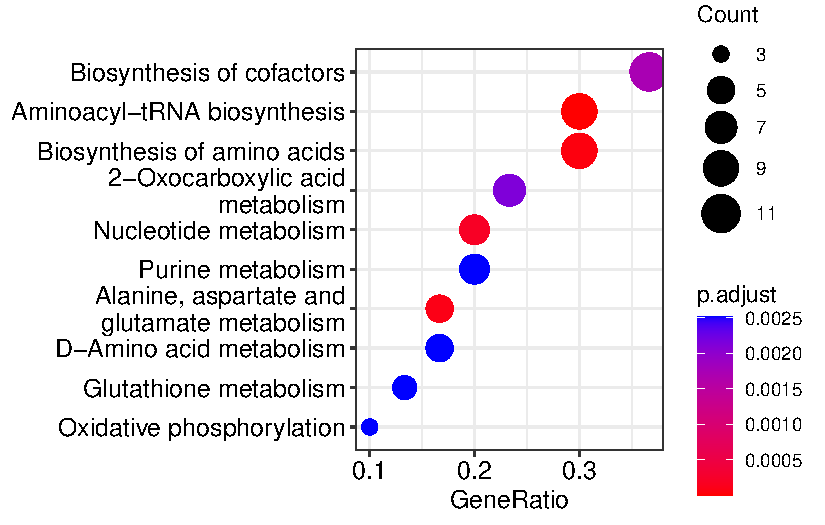
\includegraphics{index_files/figure-pdf/unnamed-chunk-24-1.pdf}

}

\end{figure}

\hypertarget{varying-mingssize}{%
\subsection{Varying minGSSize}\label{varying-mingssize}}

By default, ORA filters out pathways smaller than 10 metabolites when
enriching. This parameter can be varied depending on the pathway sets:
if you know that they are smaller in general, lowering this threshold
may be more relevant.

A lower minGSSize means more pathways to test against, which usually
means higher p-values but more possibilities for small pathways to be
enriched.

\begin{Shaded}
\begin{Highlighting}[]
\NormalTok{pathway.sizes }\OtherTok{=}\NormalTok{ kegg.pathways }\SpecialCharTok{\%\textgreater{}\%} \FunctionTok{group\_by}\NormalTok{(value.x) }\SpecialCharTok{\%\textgreater{}\%} \FunctionTok{summarise}\NormalTok{(}\AttributeTok{count =} \FunctionTok{n}\NormalTok{()) }
\NormalTok{pathway.counts }\OtherTok{=}\NormalTok{ pathway.sizes }\SpecialCharTok{\%\textgreater{}\%} \FunctionTok{pull}\NormalTok{(count)}
\FunctionTok{hist}\NormalTok{(pathway.counts, }\AttributeTok{breaks =} \DecValTok{50}\NormalTok{)}
\FunctionTok{abline}\NormalTok{(}\AttributeTok{v=}\DecValTok{10}\NormalTok{,}\AttributeTok{col=}\StringTok{"red"}\NormalTok{)}
\end{Highlighting}
\end{Shaded}

\begin{figure}[H]

{\centering 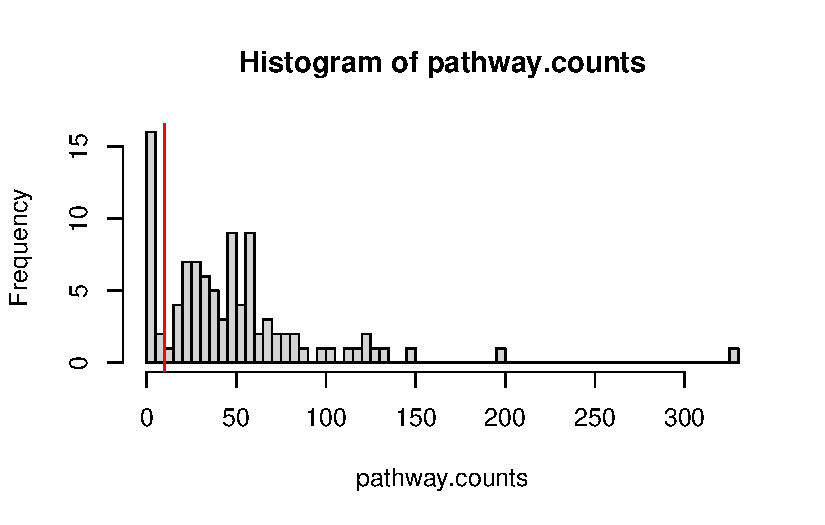
\includegraphics{index_files/figure-pdf/unnamed-chunk-25-1.pdf}

}

\end{figure}

\begin{center}\rule{0.5\linewidth}{0.5pt}\end{center}

\begin{Shaded}
\begin{Highlighting}[]
\NormalTok{ora.gestation.filtered.kegg }\OtherTok{=} \FunctionTok{enricher}\NormalTok{(geno.mother.raw}\SpecialCharTok{$}\NormalTok{KEGG , }
                                       \AttributeTok{TERM2GENE =}\NormalTok{ kegg.pathways }\SpecialCharTok{\%\textgreater{}\%} \FunctionTok{select}\NormalTok{(}\SpecialCharTok{{-}}\NormalTok{name), }
                                       \AttributeTok{minGSSize =} \DecValTok{10}\NormalTok{, }
                                       \AttributeTok{universe =}\NormalTok{ annot.db }\SpecialCharTok{\%\textgreater{}\%} \FunctionTok{pull}\NormalTok{(KEGG), }\AttributeTok{pvalueCutoff =} \FloatTok{0.1}\NormalTok{)}
\FunctionTok{dotplot}\NormalTok{(ora.gestation.filtered.kegg)}
\end{Highlighting}
\end{Shaded}

\begin{figure}[H]

{\centering 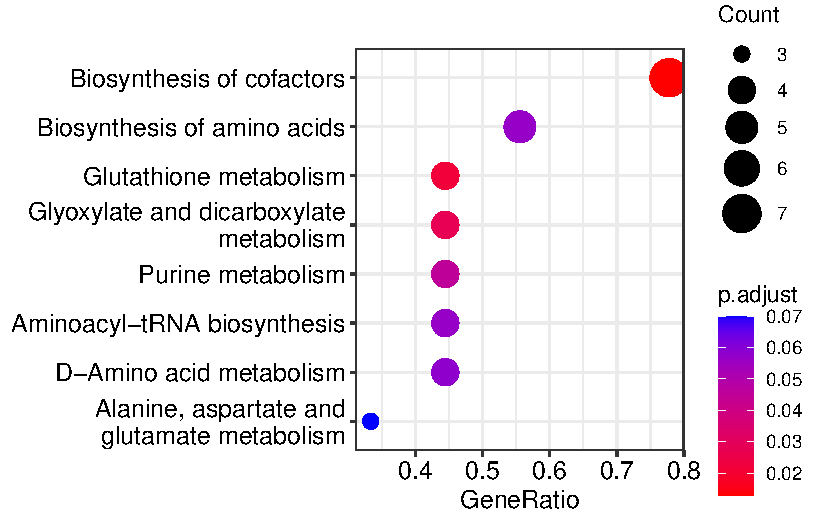
\includegraphics{index_files/figure-pdf/unnamed-chunk-26-1.pdf}

}

\end{figure}

\begin{center}\rule{0.5\linewidth}{0.5pt}\end{center}

In this case, by setting \texttt{minGSSize} to 3, we gain some new
enriched pathways at the cost of higher adjusted p-values. These
pathways weren't enriched before because there were less total pathways,
so their enrichments weren't as significant. We most likely added many
small pathways with no enrichment by lowering the \texttt{minGSSize}.

\begin{Shaded}
\begin{Highlighting}[]
\NormalTok{ora.gestation.filtered.kegg }\OtherTok{=} \FunctionTok{enricher}\NormalTok{(geno.mother.raw}\SpecialCharTok{$}\NormalTok{KEGG , }
                                       \AttributeTok{TERM2GENE =}\NormalTok{ kegg.pathways }\SpecialCharTok{\%\textgreater{}\%} \FunctionTok{select}\NormalTok{(}\SpecialCharTok{{-}}\NormalTok{name), }
                                       \AttributeTok{minGSSize =} \DecValTok{3}\NormalTok{, }
                                       \AttributeTok{universe =}\NormalTok{  annot.db }\SpecialCharTok{\%\textgreater{}\%} \FunctionTok{pull}\NormalTok{(KEGG), }\AttributeTok{pvalueCutoff =} \FloatTok{0.1}\NormalTok{)}
\FunctionTok{dotplot}\NormalTok{(ora.gestation.filtered.kegg)}
\end{Highlighting}
\end{Shaded}

\begin{figure}[H]

{\centering 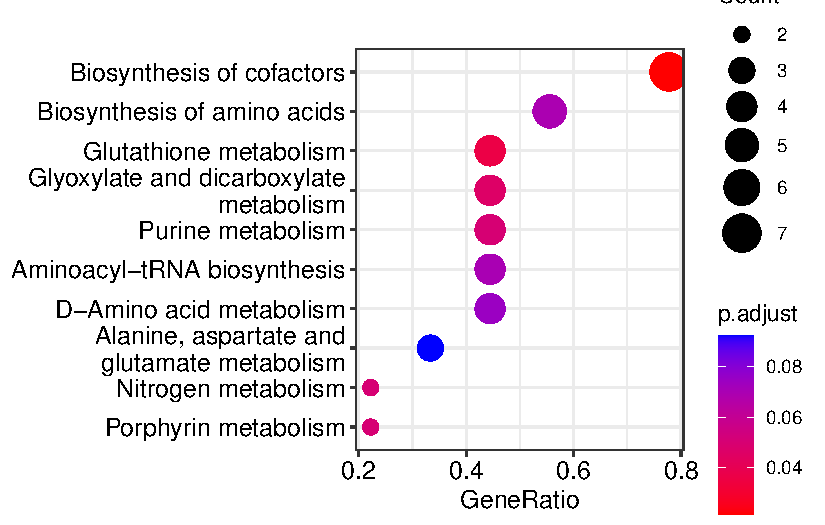
\includegraphics{index_files/figure-pdf/unnamed-chunk-27-1.pdf}

}

\end{figure}

\hypertarget{bonus-varying-p-value-cutoff}{%
\subsection{Bonus: varying p-value
cutoff}\label{bonus-varying-p-value-cutoff}}

We can also vary the p-value and p-value adjust cutoff to determine what
is and isn't a significantly enriched pathway. This must be done with
caution as a high cutoff will provide many false positives.

We can use the previous example with a \texttt{pvalueCutoff} of 0.05
(the default).

\begin{Shaded}
\begin{Highlighting}[]
\NormalTok{ora.gestation.filtered.kegg }\OtherTok{=} \FunctionTok{enricher}\NormalTok{(geno.mother.raw}\SpecialCharTok{$}\NormalTok{KEGG , }
                                       \AttributeTok{TERM2GENE =}\NormalTok{ kegg.pathways }\SpecialCharTok{\%\textgreater{}\%} \FunctionTok{select}\NormalTok{(}\SpecialCharTok{{-}}\NormalTok{name), }
                                       \AttributeTok{minGSSize =} \DecValTok{3}\NormalTok{, }
                                       \AttributeTok{universe =}\NormalTok{  annot.db }\SpecialCharTok{\%\textgreater{}\%} \FunctionTok{pull}\NormalTok{(KEGG), }\AttributeTok{pvalueCutoff =} \FloatTok{0.05}\NormalTok{)}
\FunctionTok{dotplot}\NormalTok{(ora.gestation.filtered.kegg)}
\end{Highlighting}
\end{Shaded}

\begin{figure}[H]

{\centering 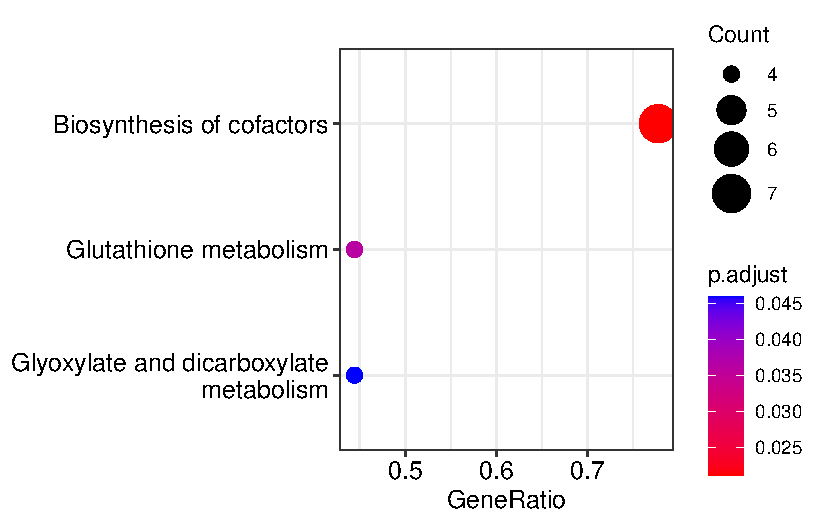
\includegraphics{index_files/figure-pdf/unnamed-chunk-28-1.pdf}

}

\end{figure}

\hypertarget{ora-on-up-vs-down-regulated-in-dataset}{%
\subsection{ORA on up vs down regulated in
dataset}\label{ora-on-up-vs-down-regulated-in-dataset}}

In addition to using the entire filtered fold changes, we can split the
dataset into up and down regulated metabolites.

\begin{Shaded}
\begin{Highlighting}[]
\NormalTok{geno.mother.raw.up }\OtherTok{=}\NormalTok{ geno.mother.raw }\SpecialCharTok{\%\textgreater{}\%} \FunctionTok{filter}\NormalTok{(log2FC\_mg }\SpecialCharTok{\textgreater{}} \DecValTok{0}\NormalTok{)}
\NormalTok{geno.mother.raw.down }\OtherTok{=}\NormalTok{ geno.mother.raw }\SpecialCharTok{\%\textgreater{}\%} \FunctionTok{filter}\NormalTok{(log2FC\_mg }\SpecialCharTok{\textless{}} \DecValTok{0}\NormalTok{)}
\end{Highlighting}
\end{Shaded}

Using a higher \texttt{pvalueCutoff} to show enriched pathways: again,
because we are being stringent with the background set and by splitting
the input set into two, we can be less strict with the p.adjust.

\hypertarget{upregulated-metabolites}{%
\subsubsection{Upregulated metabolites}\label{upregulated-metabolites}}

\begin{Shaded}
\begin{Highlighting}[]
\NormalTok{ora.geno.mother.kegg.up }\OtherTok{=} \FunctionTok{enricher}\NormalTok{(geno.mother.raw.up}\SpecialCharTok{$}\NormalTok{KEGG , }\AttributeTok{TERM2GENE =}\NormalTok{ kegg.pathways }\SpecialCharTok{\%\textgreater{}\%} \FunctionTok{select}\NormalTok{(}\SpecialCharTok{{-}}\NormalTok{name),}
                                \AttributeTok{universe =}\NormalTok{ annot.db }\SpecialCharTok{\%\textgreater{}\%} \FunctionTok{pull}\NormalTok{(KEGG), }\AttributeTok{pvalueCutoff =} \FloatTok{0.2}\NormalTok{, }\AttributeTok{minGSSize =} \DecValTok{3}\NormalTok{)}
\FunctionTok{dotplot}\NormalTok{(ora.geno.mother.kegg.up)}
\end{Highlighting}
\end{Shaded}

\begin{figure}[H]

{\centering 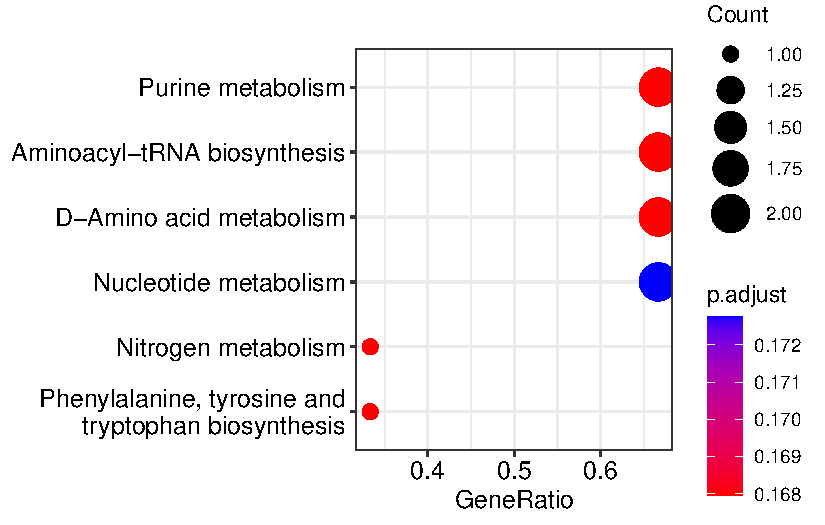
\includegraphics{index_files/figure-pdf/unnamed-chunk-30-1.pdf}

}

\end{figure}

\begin{center}\rule{0.5\linewidth}{0.5pt}\end{center}

We can plot using the p-value as a the colour to show that these
unadjusted p-values are still significant.

\begin{Shaded}
\begin{Highlighting}[]
\FunctionTok{dotplot}\NormalTok{(ora.geno.mother.kegg.up, }\AttributeTok{color =} \StringTok{"pvalue"}\NormalTok{)}
\end{Highlighting}
\end{Shaded}

\begin{figure}[H]

{\centering 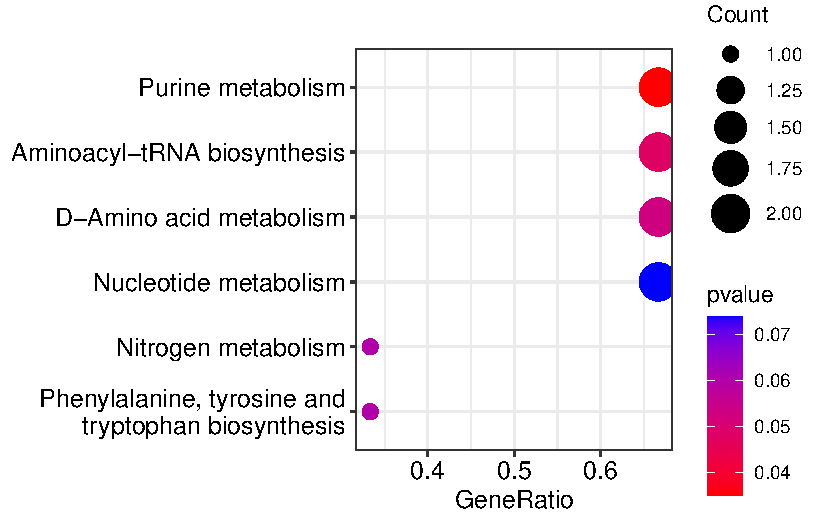
\includegraphics{index_files/figure-pdf/unnamed-chunk-31-1.pdf}

}

\end{figure}

\begin{center}\rule{0.5\linewidth}{0.5pt}\end{center}

\hypertarget{downregulated-metabolites}{%
\subsubsection{Downregulated
metabolites:}\label{downregulated-metabolites}}

\begin{Shaded}
\begin{Highlighting}[]
\NormalTok{ora.geno.mother.kegg.down }\OtherTok{=} \FunctionTok{enricher}\NormalTok{(geno.mother.raw.down}\SpecialCharTok{$}\NormalTok{KEGG , }\AttributeTok{TERM2GENE =}\NormalTok{ kegg.pathways }\SpecialCharTok{\%\textgreater{}\%} \FunctionTok{select}\NormalTok{(}\SpecialCharTok{{-}}\NormalTok{name),}
                                \AttributeTok{universe =}\NormalTok{ annot.db }\SpecialCharTok{\%\textgreater{}\%} \FunctionTok{pull}\NormalTok{(KEGG), }\AttributeTok{pvalueCutoff =} \FloatTok{0.1}\NormalTok{, }\AttributeTok{minGSSize =} \DecValTok{3}\NormalTok{)}
\FunctionTok{dotplot}\NormalTok{(ora.geno.mother.kegg.down)}
\end{Highlighting}
\end{Shaded}

\begin{figure}[H]

{\centering 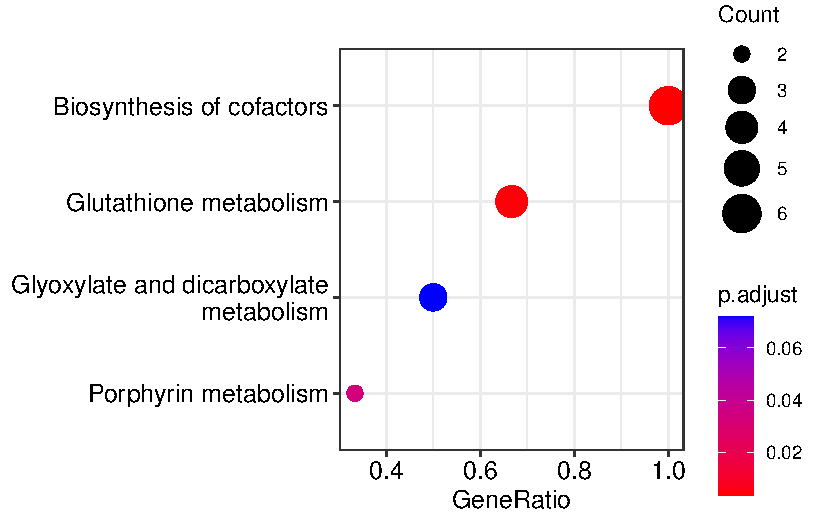
\includegraphics{index_files/figure-pdf/unnamed-chunk-32-1.pdf}

}

\end{figure}

This results in pathways that we can define as up or down regulated in
addition to being enriched.

\hypertarget{gsea}{%
\section{GSEA}\label{gsea}}

In this section, we remove set multiple correction to \texttt{"none"} as
GSEA will not return anything significant with a small input dataset.
This is illustrated using the gseaplots.

\hypertarget{gestation-data-set-1}{%
\subsection{Gestation data set}\label{gestation-data-set-1}}

\hypertarget{using-fold-changes}{%
\subsubsection{Using fold changes}\label{using-fold-changes}}

For illustrative purposes, we set the \texttt{pvalueCutoff} to be 1 to
show all pathway p-values.

\begin{Shaded}
\begin{Highlighting}[]
\NormalTok{gsea.input.gestation }\OtherTok{=}\NormalTok{ all.fc }\SpecialCharTok{\%\textgreater{}\%} 
  \FunctionTok{arrange}\NormalTok{(}\FunctionTok{desc}\NormalTok{(gestation)) }\SpecialCharTok{\%\textgreater{}\%} 
  \FunctionTok{na.omit}\NormalTok{() }\SpecialCharTok{\%\textgreater{}\%}
  \FunctionTok{pull}\NormalTok{(gestation,KEGG) }

\NormalTok{gsea.gestation.kegg }\OtherTok{=} \FunctionTok{GSEA}\NormalTok{(gsea.input.gestation, }
                           \AttributeTok{TERM2GENE =}\NormalTok{ kegg.pathways }\SpecialCharTok{\%\textgreater{}\%} \FunctionTok{select}\NormalTok{(}\SpecialCharTok{{-}}\NormalTok{name),}
                           \AttributeTok{minGSSize =} \DecValTok{3}\NormalTok{, }\AttributeTok{pvalueCutoff =} \DecValTok{1}\NormalTok{,}
                           \AttributeTok{pAdjustMethod =} \StringTok{"none"}\NormalTok{)}
\end{Highlighting}
\end{Shaded}

\begin{verbatim}
preparing geneSet collections...
\end{verbatim}

\begin{verbatim}
GSEA analysis...
\end{verbatim}

\begin{verbatim}
leading edge analysis...
\end{verbatim}

\begin{verbatim}
done...
\end{verbatim}

\begin{Shaded}
\begin{Highlighting}[]
\FunctionTok{tibble}\NormalTok{(gsea.gestation.kegg}\SpecialCharTok{@}\NormalTok{result)}
\end{Highlighting}
\end{Shaded}

\begin{verbatim}
# A tibble: 27 x 11
   ID     Description setSize enrichmentScore   NES pvalue p.adjust qvalue  rank
   <chr>  <chr>         <int>           <dbl> <dbl>  <dbl>    <dbl>  <dbl> <dbl>
 1 Purin~ Purine met~       7          -0.731 -1.30  0.134    0.134  0.966     9
 2 Nucle~ Nucleotide~       6          -0.740 -1.28  0.136    0.136  0.966     9
 3 Cyste~ Cysteine a~       5           0.652  1.24  0.249    0.249  0.966     1
 4 Pheny~ Phenylalan~       4           0.670  1.20  0.290    0.290  0.966    10
 5 Tyros~ Tyrosine m~       3           0.726  1.20  0.309    0.309  0.966     6
 6 Sulfu~ Sulfur met~       4           0.632  1.14  0.362    0.362  0.966     6
 7 Valin~ Valine, le~       3           0.683  1.13  0.385    0.385  0.966    16
 8 Valin~ Valine, le~       3           0.683  1.13  0.385    0.385  0.966    16
 9 Argin~ Arginine b~       3          -0.732 -1.10  0.416    0.416  0.966    15
10 Pyruv~ Pyruvate m~       3           0.658  1.09  0.431    0.431  0.966    12
# i 17 more rows
# i 2 more variables: leading_edge <chr>, core_enrichment <chr>
\end{verbatim}

\begin{center}\rule{0.5\linewidth}{0.5pt}\end{center}

This gseaplot shows that even if Purine metabolism seems to be enriched,
with so few metabolites it doesn't reach a high enough enrichment score
and p-value to be classed as significant when correcting the p-value.
Even the raw p-value is fairly high at 0.169.

The gseaplot also reveals that we have a split of strong fold changed
metabolites: 1 up and 4 down.

\begin{Shaded}
\begin{Highlighting}[]
\NormalTok{enrichplot}\SpecialCharTok{::}\FunctionTok{gseaplot2}\NormalTok{(gsea.gestation.kegg, }\AttributeTok{geneSetID =} \DecValTok{1}\NormalTok{, }\AttributeTok{title =}\NormalTok{ gsea.gestation.kegg}\SpecialCharTok{$}\NormalTok{Description[}\DecValTok{1}\NormalTok{])}
\end{Highlighting}
\end{Shaded}

\begin{figure}[H]

{\centering 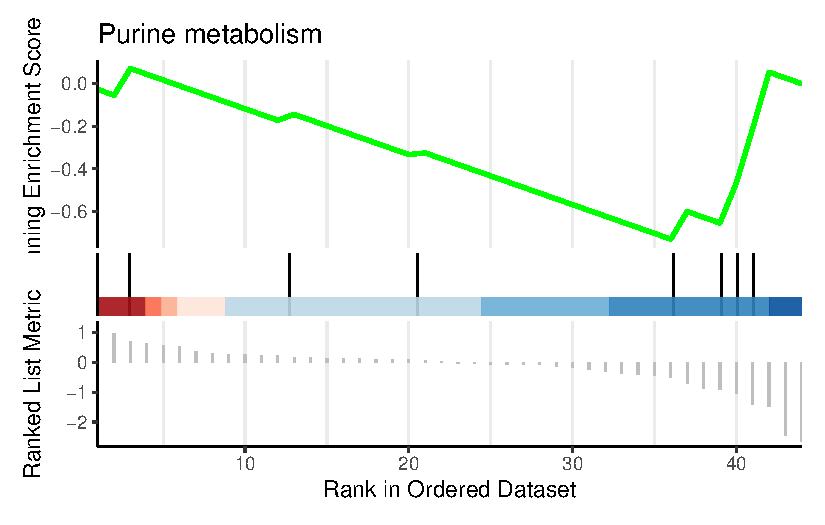
\includegraphics{index_files/figure-pdf/unnamed-chunk-34-1.pdf}

}

\end{figure}

\begin{center}\rule{0.5\linewidth}{0.5pt}\end{center}

This dotplot uses the unadjusted pvalue as the colour legend. Only the
very red pathways could be considered as enriched.

\begin{Shaded}
\begin{Highlighting}[]
\FunctionTok{dotplot}\NormalTok{(gsea.gestation.kegg, }\AttributeTok{color =} \StringTok{"pvalue"}\NormalTok{)}
\end{Highlighting}
\end{Shaded}

\begin{figure}[H]

{\centering 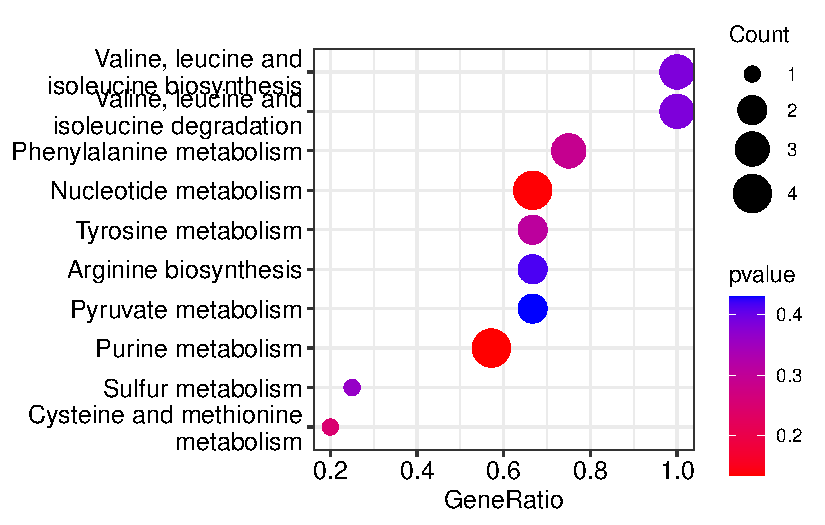
\includegraphics{index_files/figure-pdf/unnamed-chunk-35-1.pdf}

}

\end{figure}

\begin{center}\rule{0.5\linewidth}{0.5pt}\end{center}

\hypertarget{using-absolute-fold-changes}{%
\subsubsection{Using absolute fold
changes}\label{using-absolute-fold-changes}}

In genomics, when genes are upregulated together this usually means that
the enriched pathway is upregulated. With metabolites, pathways can be
enriched regardless of an increase or a decrease in metabolite
concentration: this means we can look for enriched pathways that are
affected using the metabolites, without being able to conclude on its up
or down regulation.

To do this, we use the absolute value of the fold changes instead of the
raw fold changes. We also need to add a parameter to GSEA:
\texttt{scoreType\ =\ "pos"}, to do a one tailed test, since all our
values will be positive.

\begin{Shaded}
\begin{Highlighting}[]
\NormalTok{gsea.input.gestation }\OtherTok{=}\NormalTok{ all.fc }\SpecialCharTok{\%\textgreater{}\%}
  \FunctionTok{mutate}\NormalTok{(}\AttributeTok{gestation =} \FunctionTok{abs}\NormalTok{(gestation)) }\SpecialCharTok{\%\textgreater{}\%} 
  \FunctionTok{arrange}\NormalTok{(}\FunctionTok{desc}\NormalTok{(gestation)) }\SpecialCharTok{\%\textgreater{}\%} 
  \FunctionTok{na.omit}\NormalTok{() }\SpecialCharTok{\%\textgreater{}\%}
  \FunctionTok{pull}\NormalTok{(gestation,KEGG) }

\NormalTok{gsea.gestation.kegg }\OtherTok{=} \FunctionTok{GSEA}\NormalTok{(gsea.input.gestation, }
                           \AttributeTok{TERM2GENE =}\NormalTok{ kegg.pathways }\SpecialCharTok{\%\textgreater{}\%} \FunctionTok{select}\NormalTok{(}\SpecialCharTok{{-}}\NormalTok{name),}
                           \AttributeTok{minGSSize =} \DecValTok{3}\NormalTok{, }\AttributeTok{pvalueCutoff =} \DecValTok{1}\NormalTok{,}
                           \AttributeTok{pAdjustMethod =} \StringTok{"none"}\NormalTok{, }
                           \AttributeTok{scoreType=}\StringTok{"pos"}\NormalTok{)}
\end{Highlighting}
\end{Shaded}

\begin{verbatim}
preparing geneSet collections...
\end{verbatim}

\begin{verbatim}
GSEA analysis...
\end{verbatim}

\begin{verbatim}
leading edge analysis...
\end{verbatim}

\begin{verbatim}
done...
\end{verbatim}

\begin{center}\rule{0.5\linewidth}{0.5pt}\end{center}

\begin{Shaded}
\begin{Highlighting}[]
\NormalTok{enrichplot}\SpecialCharTok{::}\FunctionTok{gseaplot2}\NormalTok{(gsea.gestation.kegg, }\AttributeTok{geneSetID =} \DecValTok{1}\NormalTok{, }\AttributeTok{title =}\NormalTok{ gsea.gestation.kegg}\SpecialCharTok{$}\NormalTok{Description[}\DecValTok{1}\NormalTok{])}
\end{Highlighting}
\end{Shaded}

\begin{figure}[H]

{\centering 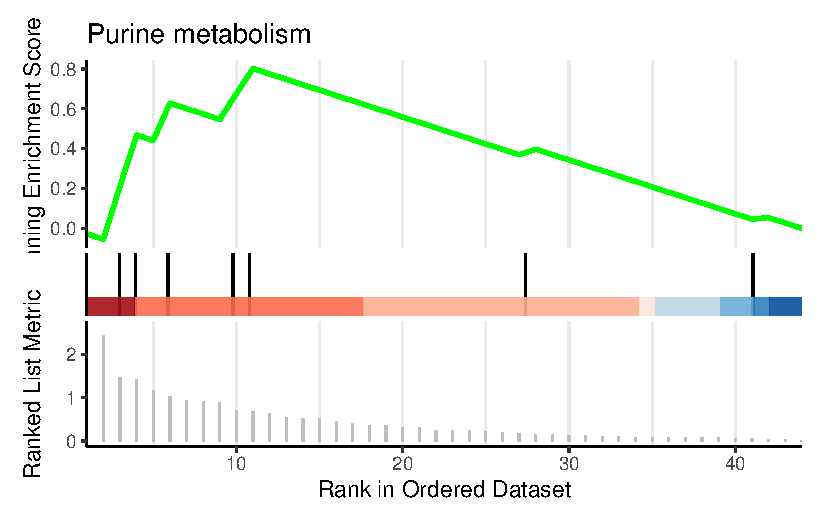
\includegraphics{index_files/figure-pdf/unnamed-chunk-37-1.pdf}

}

\end{figure}

In the gseaplot, we can see that we have 5 highly ranked metabolites for
Purine metabolism, instead of 1 up and 4 down as seen in the previous
gseaplot. This groups together the metabolites affected by the condition
in order to better enrich affected pathways.

\hypertarget{geno-mother-data-set}{%
\subsection{Geno mother data set}\label{geno-mother-data-set}}

We can do the same analyses with the second data set.

\hypertarget{using-fold-changes-1}{%
\subsubsection{Using fold changes}\label{using-fold-changes-1}}

\begin{Shaded}
\begin{Highlighting}[]
\NormalTok{gsea.input.geno }\OtherTok{=}\NormalTok{ all.fc }\SpecialCharTok{\%\textgreater{}\%}
  \FunctionTok{mutate}\NormalTok{(}\AttributeTok{geno.mother =}\NormalTok{ geno.mother) }\SpecialCharTok{\%\textgreater{}\%} 
  \FunctionTok{arrange}\NormalTok{(}\FunctionTok{desc}\NormalTok{(geno.mother))}\SpecialCharTok{\%\textgreater{}\%} \FunctionTok{na.omit}\NormalTok{() }\SpecialCharTok{\%\textgreater{}\%}
  \FunctionTok{pull}\NormalTok{(geno.mother,KEGG) }

\NormalTok{gsea.geno.kegg }\OtherTok{=} \FunctionTok{GSEA}\NormalTok{(gsea.input.geno, }
                      \AttributeTok{TERM2GENE =}\NormalTok{ kegg.pathways }\SpecialCharTok{\%\textgreater{}\%} \FunctionTok{select}\NormalTok{(}\SpecialCharTok{{-}}\NormalTok{name),}
                      \AttributeTok{minGSSize =} \DecValTok{3}\NormalTok{, }
                      \AttributeTok{pvalueCutoff =} \DecValTok{1}\NormalTok{, }
                      \AttributeTok{pAdjustMethod =} \StringTok{"none"}\NormalTok{)}
\end{Highlighting}
\end{Shaded}

\begin{verbatim}
preparing geneSet collections...
\end{verbatim}

\begin{verbatim}
GSEA analysis...
\end{verbatim}

\begin{verbatim}
leading edge analysis...
\end{verbatim}

\begin{verbatim}
done...
\end{verbatim}

\begin{Shaded}
\begin{Highlighting}[]
\FunctionTok{tibble}\NormalTok{(gsea.geno.kegg}\SpecialCharTok{@}\NormalTok{result)}
\end{Highlighting}
\end{Shaded}

\begin{verbatim}
# A tibble: 27 x 11
   ID    Description setSize enrichmentScore   NES  pvalue p.adjust qvalue  rank
   <chr> <chr>         <int>           <dbl> <dbl>   <dbl>    <dbl>  <dbl> <dbl>
 1 Bios~ Biosynthes~      14          -0.718 -1.61 0.00706  0.00706  0.191    12
 2 Thia~ Thiamine m~       3          -0.902 -1.44 0.0546   0.0546   0.626     8
 3 Cyst~ Cysteine a~       5          -0.808 -1.44 0.0696   0.0696   0.626     3
 4 Glut~ Glutathion~       5          -0.783 -1.40 0.0994   0.0994   0.671    12
 5 Carb~ Carbon met~       9          -0.587 -1.20 0.257    0.257    0.972    13
 6 Oxid~ Oxidative ~       3          -0.749 -1.19 0.311    0.311    0.972     8
 7 Glyc~ Glyceropho~       5           0.688  1.18 0.347    0.347    0.972    15
 8 Nucl~ Nucleotide~       6           0.610  1.09 0.426    0.426    0.972     4
 9 Puri~ Purine met~       7           0.571  1.06 0.428    0.428    0.972     4
10 Argi~ Arginine b~       3           0.671  1.07 0.463    0.463    0.972     3
# i 17 more rows
# i 2 more variables: leading_edge <chr>, core_enrichment <chr>
\end{verbatim}

\begin{center}\rule{0.5\linewidth}{0.5pt}\end{center}

\begin{Shaded}
\begin{Highlighting}[]
\FunctionTok{dotplot}\NormalTok{(gsea.geno.kegg)}
\end{Highlighting}
\end{Shaded}

\begin{figure}[H]

{\centering 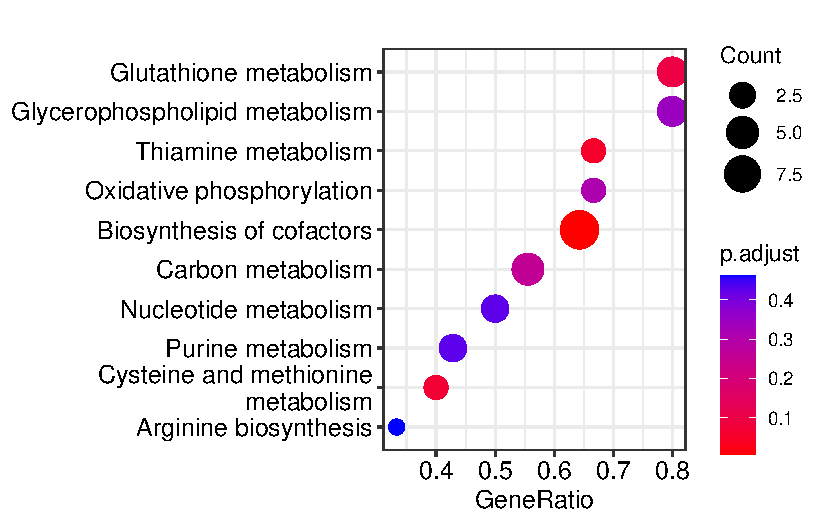
\includegraphics{index_files/figure-pdf/unnamed-chunk-39-1.pdf}

}

\end{figure}

\begin{center}\rule{0.5\linewidth}{0.5pt}\end{center}

The most enriched pathway for this dataset is Biosynthesis of cofactors.
In the gseaplot, many metabolites have a strong negative fold change.

\begin{Shaded}
\begin{Highlighting}[]
\NormalTok{enrichplot}\SpecialCharTok{::}\FunctionTok{gseaplot2}\NormalTok{(gsea.geno.kegg, }\AttributeTok{geneSetID =} \DecValTok{1}\NormalTok{, }\AttributeTok{title =}\NormalTok{ gsea.geno.kegg}\SpecialCharTok{$}\NormalTok{Description[}\DecValTok{1}\NormalTok{])}
\end{Highlighting}
\end{Shaded}

\begin{figure}[H]

{\centering 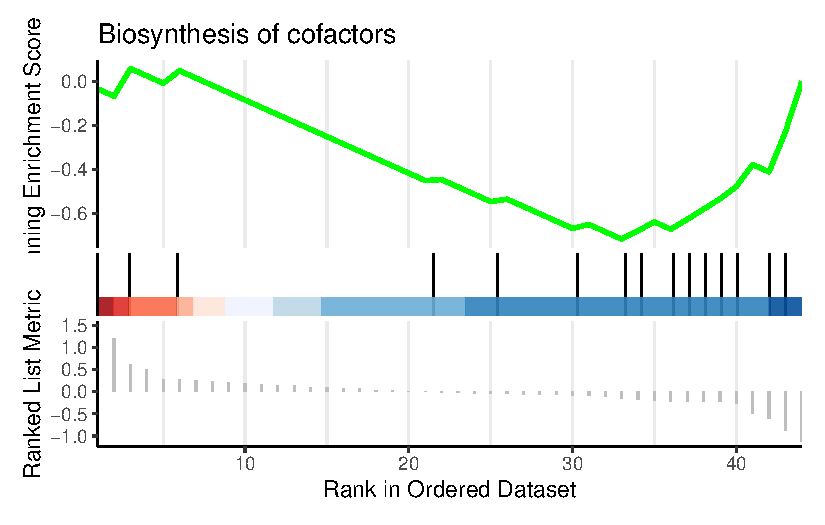
\includegraphics{index_files/figure-pdf/unnamed-chunk-40-1.pdf}

}

\end{figure}

\begin{center}\rule{0.5\linewidth}{0.5pt}\end{center}

\hypertarget{using-absolute-fold-changes-1}{%
\subsubsection{Using absolute fold
changes}\label{using-absolute-fold-changes-1}}

By using the absolute values of fold changes, we can reveal pathways
that weren't enriched before simply because their metabolites were split
over up and down regulated metabolites.

\begin{Shaded}
\begin{Highlighting}[]
\NormalTok{gsea.input.geno.abs }\OtherTok{=}\NormalTok{ all.fc }\SpecialCharTok{\%\textgreater{}\%}
  \FunctionTok{mutate}\NormalTok{(}\AttributeTok{geno.mother =} \FunctionTok{abs}\NormalTok{(geno.mother)) }\SpecialCharTok{\%\textgreater{}\%} 
  \FunctionTok{arrange}\NormalTok{(}\FunctionTok{desc}\NormalTok{(geno.mother)) }\SpecialCharTok{\%\textgreater{}\%} 
  \FunctionTok{na.omit}\NormalTok{() }\SpecialCharTok{\%\textgreater{}\%}
  \FunctionTok{pull}\NormalTok{(geno.mother,KEGG) }

\NormalTok{gsea.geno.kegg.abs }\OtherTok{=} \FunctionTok{GSEA}\NormalTok{(gsea.input.geno.abs, }
                           \AttributeTok{TERM2GENE =}\NormalTok{ kegg.pathways }\SpecialCharTok{\%\textgreater{}\%} \FunctionTok{select}\NormalTok{(}\SpecialCharTok{{-}}\NormalTok{name),}
                           \AttributeTok{minGSSize =} \DecValTok{3}\NormalTok{, }\AttributeTok{pvalueCutoff =} \DecValTok{1}\NormalTok{,}
                           \AttributeTok{pAdjustMethod =} \StringTok{"none"}\NormalTok{, }
                           \AttributeTok{scoreType=}\StringTok{"pos"}\NormalTok{)}
\end{Highlighting}
\end{Shaded}

\begin{verbatim}
preparing geneSet collections...
\end{verbatim}

\begin{verbatim}
GSEA analysis...
\end{verbatim}

\begin{verbatim}
leading edge analysis...
\end{verbatim}

\begin{verbatim}
done...
\end{verbatim}

\begin{center}\rule{0.5\linewidth}{0.5pt}\end{center}

\begin{Shaded}
\begin{Highlighting}[]
\NormalTok{enrichplot}\SpecialCharTok{::}\FunctionTok{gseaplot2}\NormalTok{(gsea.geno.kegg, }\AttributeTok{geneSetID =} \DecValTok{9}\NormalTok{, }\AttributeTok{title =}\NormalTok{ gsea.geno.kegg}\SpecialCharTok{$}\NormalTok{Description[}\DecValTok{9}\NormalTok{])}
\end{Highlighting}
\end{Shaded}

\begin{figure}[H]

{\centering 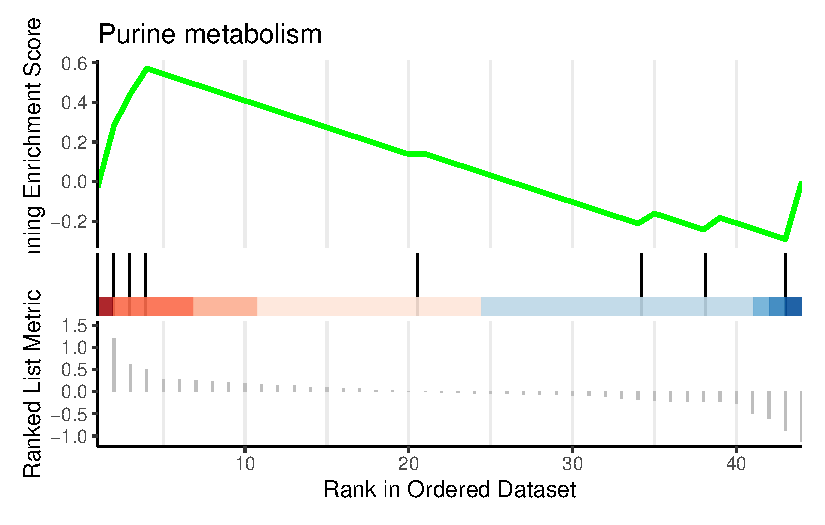
\includegraphics{index_files/figure-pdf/unnamed-chunk-42-1.pdf}

}

\end{figure}

\begin{Shaded}
\begin{Highlighting}[]
\NormalTok{enrichplot}\SpecialCharTok{::}\FunctionTok{gseaplot2}\NormalTok{(gsea.geno.kegg.abs, }\AttributeTok{geneSetID =} \DecValTok{1}\NormalTok{, }\AttributeTok{title =}\NormalTok{ gsea.geno.kegg.abs}\SpecialCharTok{$}\NormalTok{Description[}\DecValTok{1}\NormalTok{])}
\end{Highlighting}
\end{Shaded}

\begin{figure}[H]

{\centering 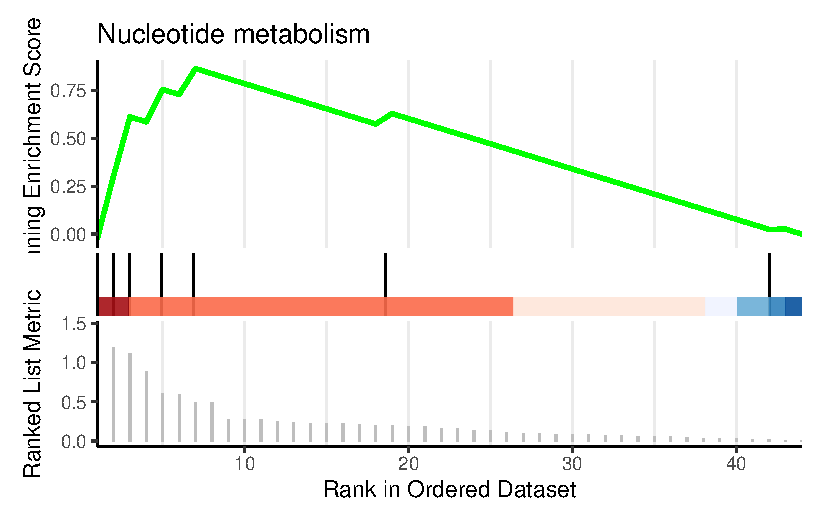
\includegraphics{index_files/figure-pdf/unnamed-chunk-42-2.pdf}

}

\end{figure}

\hypertarget{metabolic-network-pathways-instead-of-kegg-pathways}{%
\subsection{Metabolic network pathways instead of KEGG
pathways}\label{metabolic-network-pathways-instead-of-kegg-pathways}}

\begin{Shaded}
\begin{Highlighting}[]
\NormalTok{gsea.gestation.network }\OtherTok{=} \FunctionTok{GSEA}\NormalTok{(gsea.input.gestation, }
                      \AttributeTok{TERM2GENE =}\NormalTok{ metab.network.pathways }\SpecialCharTok{\%\textgreater{}\%} \FunctionTok{select}\NormalTok{(subsystem, kegg) }\SpecialCharTok{\%\textgreater{}\%} \FunctionTok{na.omit}\NormalTok{(),}
                      \AttributeTok{minGSSize =} \DecValTok{3}\NormalTok{, }\AttributeTok{pvalueCutoff =} \FloatTok{0.1}\NormalTok{, }\AttributeTok{pAdjustMethod =} \StringTok{"none"}\NormalTok{)}
\end{Highlighting}
\end{Shaded}

\begin{verbatim}
preparing geneSet collections...
\end{verbatim}

\begin{verbatim}
GSEA analysis...
\end{verbatim}

\begin{verbatim}
Warning in preparePathwaysAndStats(pathways, stats, minSize, maxSize,
gseaParam, : All values in the stats vector are greater than zero and scoreType
is "std", maybe you should switch to scoreType = "pos".
\end{verbatim}

\begin{verbatim}
leading edge analysis...
\end{verbatim}

\begin{verbatim}
done...
\end{verbatim}

\begin{Shaded}
\begin{Highlighting}[]
\FunctionTok{tibble}\NormalTok{(gsea.gestation.network}\SpecialCharTok{@}\NormalTok{result)}
\end{Highlighting}
\end{Shaded}

\begin{verbatim}
# A tibble: 1 x 11
  ID      Description setSize enrichmentScore   NES pvalue p.adjust qvalue  rank
  <chr>   <chr>         <int>           <dbl> <dbl>  <dbl>    <dbl>  <dbl> <int>
1 Purine~ Purine met~      11           0.709  1.31 0.0995   0.0995  0.961    11
# i 2 more variables: leading_edge <chr>, core_enrichment <chr>
\end{verbatim}

\begin{Shaded}
\begin{Highlighting}[]
\FunctionTok{dotplot}\NormalTok{(gsea.gestation.network)}
\end{Highlighting}
\end{Shaded}

\begin{figure}[H]

{\centering 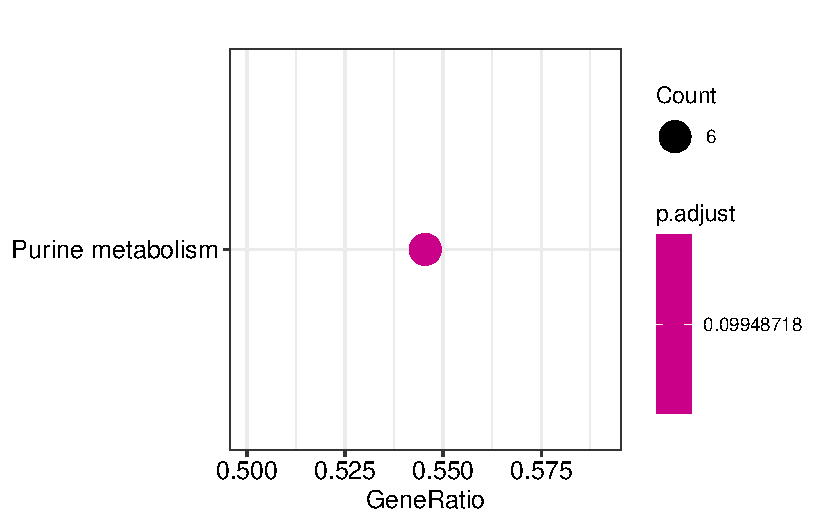
\includegraphics{index_files/figure-pdf/unnamed-chunk-43-1.pdf}

}

\end{figure}

\begin{center}\rule{0.5\linewidth}{0.5pt}\end{center}

\begin{Shaded}
\begin{Highlighting}[]
\NormalTok{enrichplot}\SpecialCharTok{::}\FunctionTok{gseaplot2}\NormalTok{(gsea.gestation.network, }\AttributeTok{geneSetID =} \DecValTok{1}\NormalTok{, }\AttributeTok{title =}\NormalTok{ gsea.gestation.network}\SpecialCharTok{$}\NormalTok{Description[}\DecValTok{1}\NormalTok{])}
\end{Highlighting}
\end{Shaded}

\begin{figure}[H]

{\centering 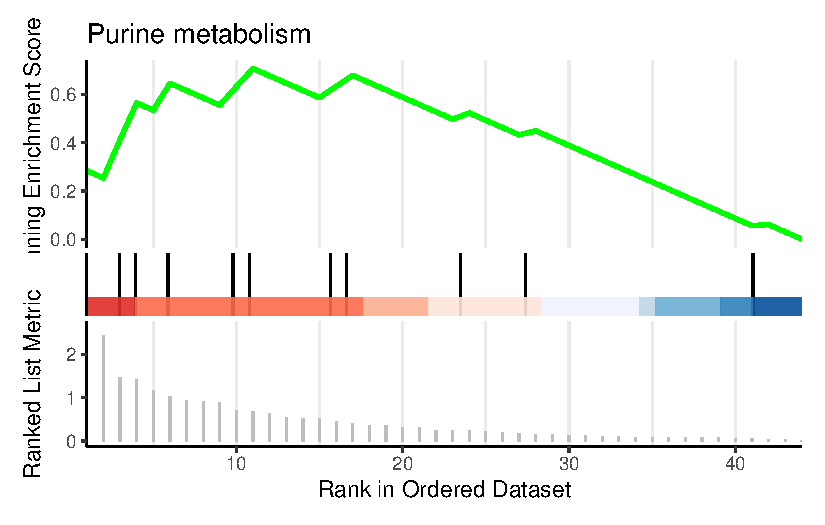
\includegraphics{index_files/figure-pdf/unnamed-chunk-44-1.pdf}

}

\end{figure}

\begin{center}\rule{0.5\linewidth}{0.5pt}\end{center}

\begin{Shaded}
\begin{Highlighting}[]
\NormalTok{gsea.geno.kegg }\OtherTok{=} \FunctionTok{GSEA}\NormalTok{(gsea.input.geno, }
                      \AttributeTok{TERM2GENE =}\NormalTok{ metab.network.pathways }\SpecialCharTok{\%\textgreater{}\%} \FunctionTok{select}\NormalTok{(subsystem, kegg) }\SpecialCharTok{\%\textgreater{}\%} \FunctionTok{na.omit}\NormalTok{(),}
                      \AttributeTok{minGSSize =} \DecValTok{3}\NormalTok{, }\AttributeTok{pvalueCutoff =} \FloatTok{0.05}\NormalTok{, }\AttributeTok{pAdjustMethod =} \StringTok{"none"}\NormalTok{)}
\end{Highlighting}
\end{Shaded}

\begin{verbatim}
preparing geneSet collections...
\end{verbatim}

\begin{verbatim}
GSEA analysis...
\end{verbatim}

\begin{verbatim}
leading edge analysis...
\end{verbatim}

\begin{verbatim}
done...
\end{verbatim}

\begin{Shaded}
\begin{Highlighting}[]
\FunctionTok{tibble}\NormalTok{(gsea.geno.kegg}\SpecialCharTok{@}\NormalTok{result)}
\end{Highlighting}
\end{Shaded}

\begin{verbatim}
# A tibble: 3 x 11
  ID      Description setSize enrichmentScore   NES pvalue p.adjust qvalue  rank
  <chr>   <chr>         <int>           <dbl> <dbl>  <dbl>    <dbl>  <dbl> <dbl>
1 Glutat~ Glutathion~       8          -0.817 -1.68 0.0137   0.0137  0.290    12
2 Ascorb~ Ascorbate ~       4          -0.9   -1.54 0.0180   0.0180  0.290     9
3 Glycin~ Glycine, s~      11          -0.736 -1.58 0.0223   0.0223  0.290    14
# i 2 more variables: leading_edge <chr>, core_enrichment <chr>
\end{verbatim}

\begin{Shaded}
\begin{Highlighting}[]
\FunctionTok{dotplot}\NormalTok{(gsea.geno.kegg)}
\end{Highlighting}
\end{Shaded}

\begin{figure}[H]

{\centering 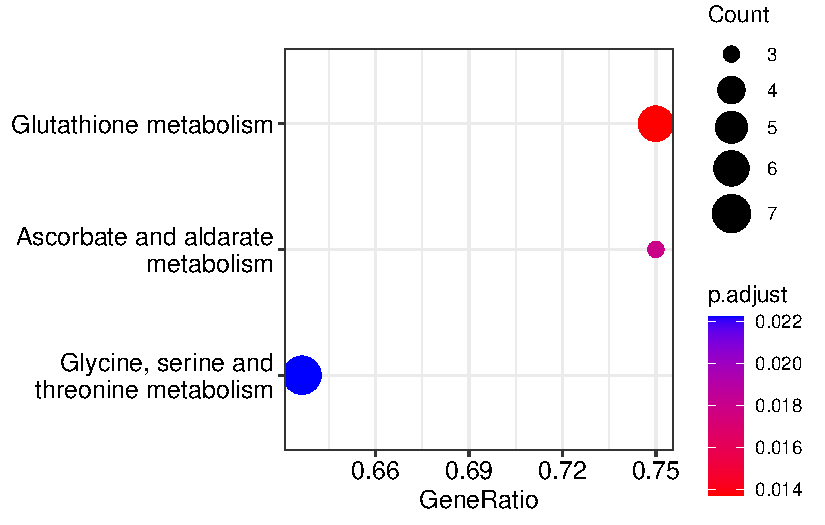
\includegraphics{index_files/figure-pdf/unnamed-chunk-45-1.pdf}

}

\end{figure}

\hypertarget{metexplore}{%
\section{MetExplore}\label{metexplore}}

MetExplore can be found
\href{https://metexplore.toulouse.inrae.fr/index.html/}{here}. Click on
START MetExplore to start.

It can be used without an account.

\hypertarget{biosource}{%
\subsection{Biosource}\label{biosource}}

In the Network Data tab, you can browse all available BioSources.
BioSources are metabolic networks. We recommend using the Human1 /
HumanGEM network as it is the most recent network.

On the right of the website, you can start typing the name of a network
and select the network you wish to use. You can also right click in the
BioSources table and Select Biosource.

\hypertarget{data-in-the-network}{%
\subsection{Data in the network}\label{data-in-the-network}}

The tabs along the top of the window in the Network Data tab show the
different types of information included in the network.


\includegraphics{images/metexplore_network_data.png}

Compartments represent cellular compartments such as cytosol,
nucleus\ldots{}

Pathways are pathway sets defined in the model.

Reactions usually have a name and a GPR (gene protein reaction)
relationship, which is a rule defining the activity of a reaction based
on the activity of one or more genes.


\includegraphics{images/metexplore_GPR.png}

Metabolites have a name and an Identifier, either specific to the
network or sometimes an external ID (KEGG for example). They also
usually have a compartment, meaning there are multiple versions of some
metabolites with different compartments.

\hypertarget{mapping-your-data}{%
\subsection{Mapping your data}\label{mapping-your-data}}

If you have reaction or metabolite IDs, you can map them to a network,
run pathway enrichment and visualise them. This is done by clicking the
Omics button \textgreater{} Mapping \textgreater{} From Omics.

Here you can upload a file or copy paste directly from Excel into the
grid. In this example, we pasted the KEGG IDs from the geno mother
dataset.

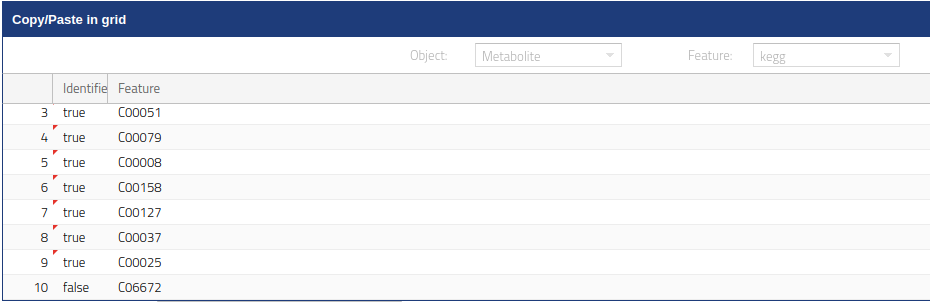
\includegraphics{images/metexplore_id_pasted.png}

\begin{center}\rule{0.5\linewidth}{0.5pt}\end{center}

By checking ``Taking into account chemical library'' you can provide a
background set for pathway enrichment. Once you have uploaded or pasted
the data, you can select the Feature type depending on the ID you
provided (e.g.~KEGG). Then, click Map, and it will tell you how many IDs
were successfully mapped to the network.


\includegraphics{images/metexplore_mapping_results.png}

\hypertarget{pathway-enrichment}{%
\subsection{Pathway enrichment}\label{pathway-enrichment}}

When data is mapped, pathway enrichment is automatically calculated on
the input data.

You can find the results in Network Data \textgreater{} Pathways as new
columns. You can then click on the column names to order by p-value,
coverage etc.

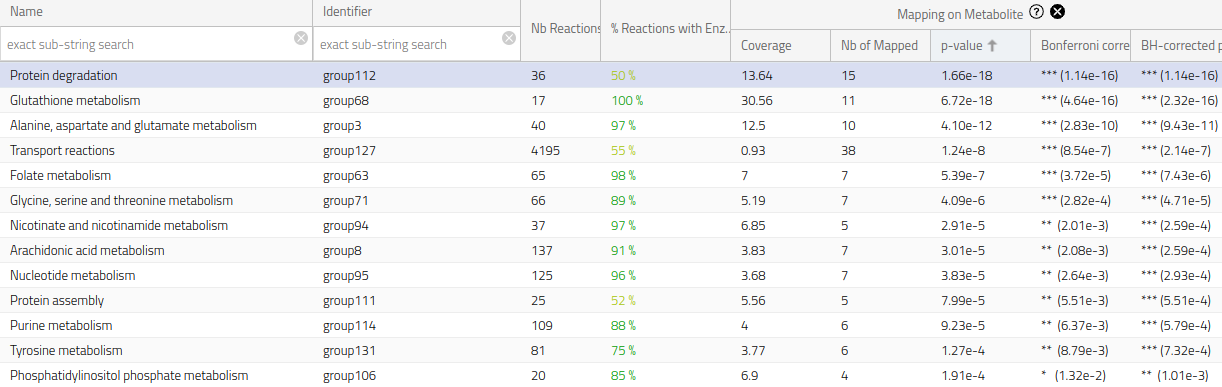
\includegraphics{images/metexplore_top_PE.png}

\hypertarget{visualise-the-selected-network}{%
\subsection{Visualise the selected
network}\label{visualise-the-selected-network}}

By selecting one or more pathways, you can visualise your mapped data
among all metabolites of the pathway(s). To do this, select multiple
pathways by Shift + clicking or Ctrl + clicking. Once you have your
selection, right click \textgreater{} Filter on selection. This will
filter the reactions in the network to only show those in the pathways
you have filtered.

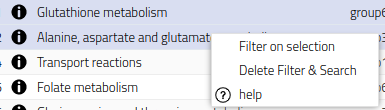
\includegraphics{images/metexplore_filter_on_selection.png}

\begin{center}\rule{0.5\linewidth}{0.5pt}\end{center}

\hypertarget{cart}{%
\subsubsection{Cart}\label{cart}}

You can then go into the Reactions tab and right click on any reaction
\textgreater{} Copy All to cart. The cart on the right of the screen is
what contains the reactions you will visualise in the visualisation
section.

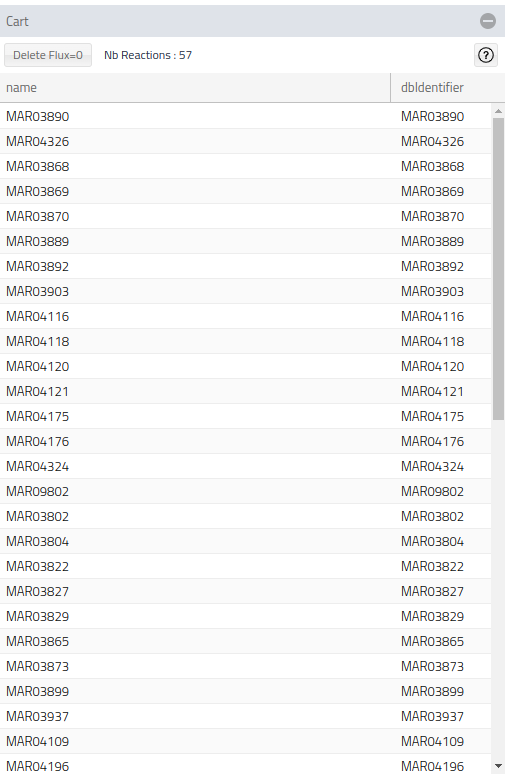
\includegraphics{images/metexplore_cart.png}

\begin{center}\rule{0.5\linewidth}{0.5pt}\end{center}

\hypertarget{create-a-network-viz}{%
\subsubsection{Create a network viz}\label{create-a-network-viz}}

Right click on any reaction in the cart and click Create network in viz
from cart, or go directly to the Network Viz tab and click MetExplore
selection.

This should show the selected reactions in the visualisation tab. Here,
metabolites are circles and reactions are squares.

\begin{figure}

{\centering 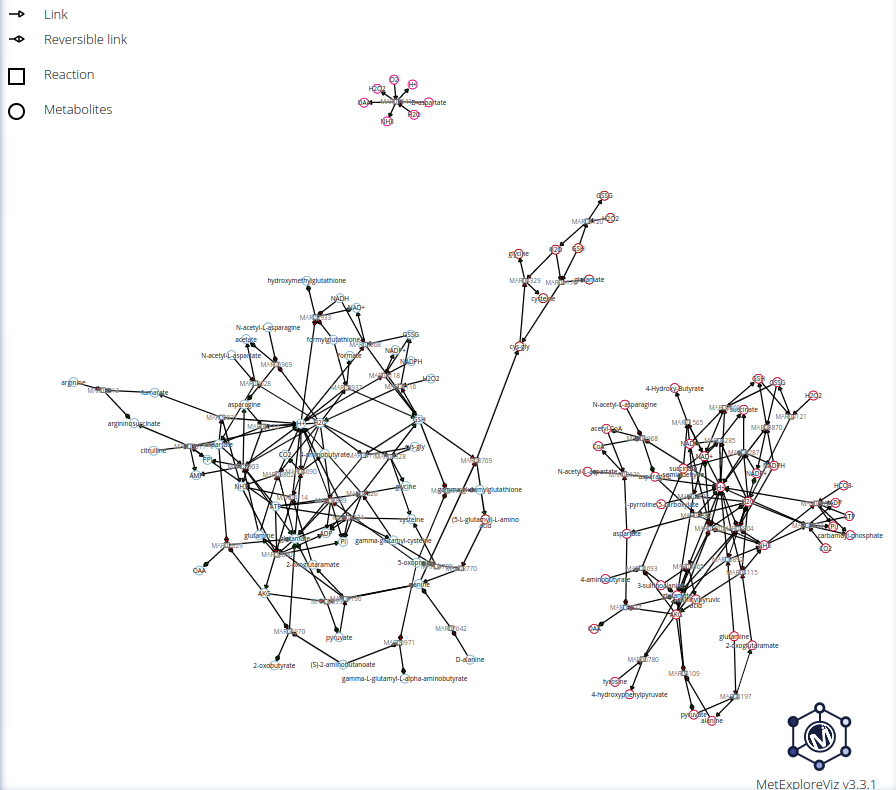
\includegraphics{images/metexplore_viz_1.png}

}

\end{figure}

\begin{center}\rule{0.5\linewidth}{0.5pt}\end{center}

\hypertarget{side-compounds}{%
\subsubsection{Side compounds}\label{side-compounds}}

Sometimes, there are some areas that are very densely connected. This is
due to side compounds being very highly connected in the network. Side
compounds are metabolites such as ATP, water, H+ used in many reactions.
In MetExplore, the Human1 metabolic network has a predefined list of
side compounds. Click on Drawing \textgreater{} Remove side compounds to
remove them from the visualisation, and click the Play button to let the
layout algorithm calculate a new layout.

\begin{figure}

{\centering 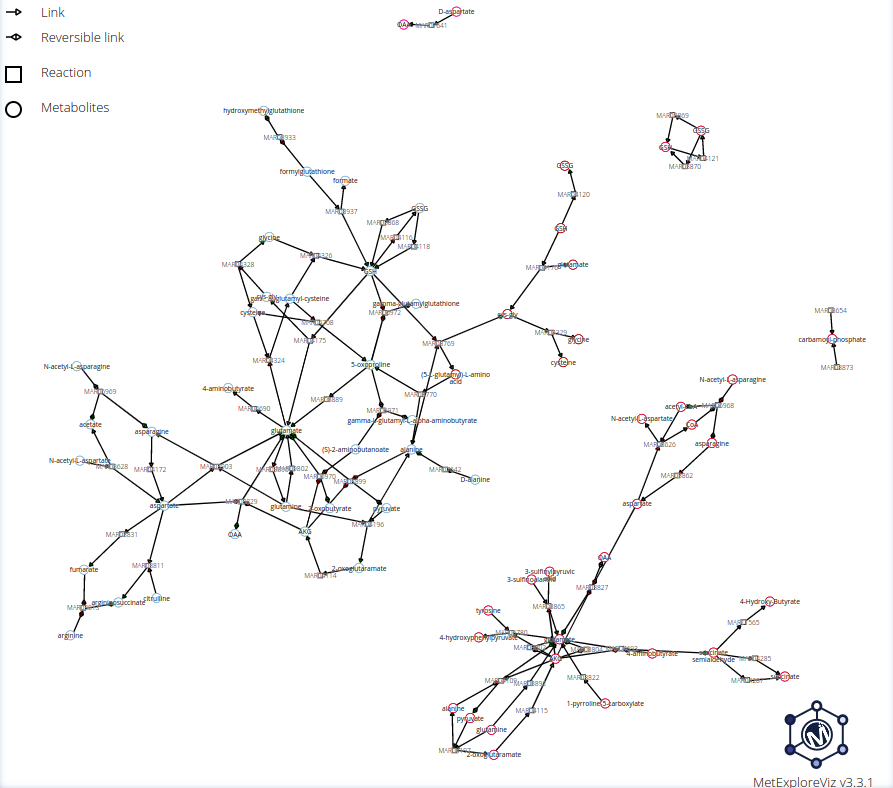
\includegraphics{images/metexplore_viz_2.png}

}

\end{figure}

\begin{center}\rule{0.5\linewidth}{0.5pt}\end{center}

\hypertarget{compartment-colours}{%
\subsubsection{Compartment colours}\label{compartment-colours}}

On the left, we have the Network Manager which helps us change various
styles of the network. Click on Compartments and click highlight
compartments on links to see the compartments for each reaction.

\begin{figure}

{\centering 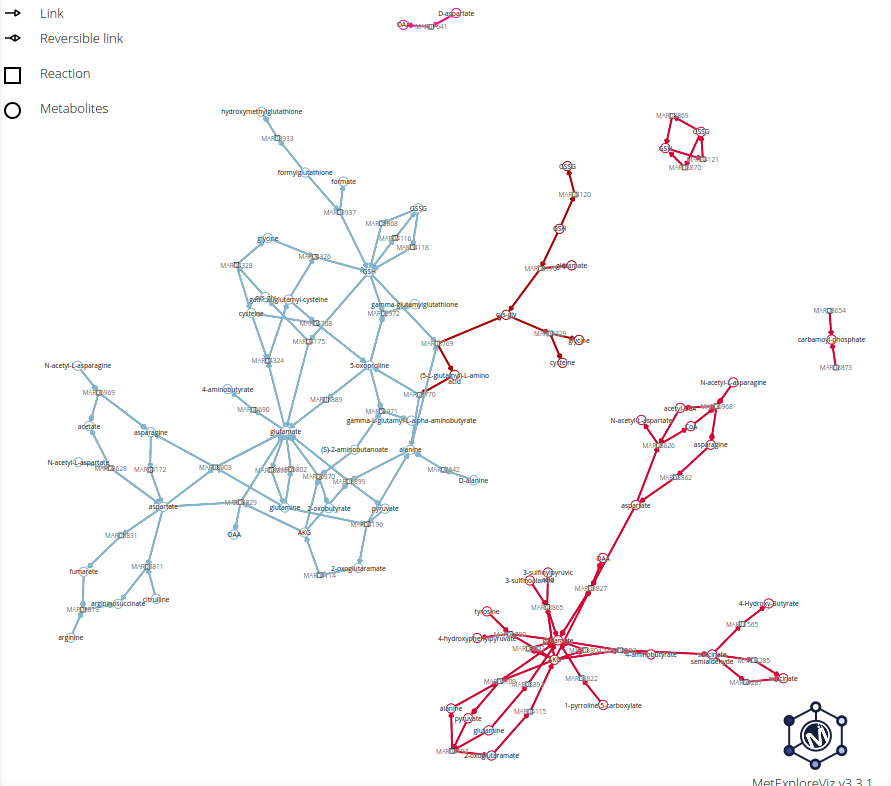
\includegraphics{images/metexplore_viz_compartments.png}

}

\end{figure}

\hypertarget{visualise-mapped-data}{%
\subsection{Visualise mapped data}\label{visualise-mapped-data}}

Go to Styles \textgreater{} Metabolite and click on the middle (Mapping)
column of the Node background. Click on Select a condition and choose
your mapping (Mapping / undefined). In Type of data, select Identified
in mapping. You can change the colour to red for example.

\begin{figure}

\begin{minipage}[t]{0.50\linewidth}

{\centering 

\raisebox{-\height}{

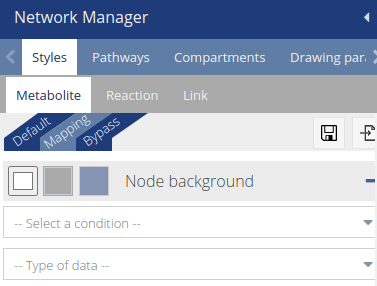
\includegraphics{images/metexplore_node_bg_select.png}

}

}

\end{minipage}%
%
\begin{minipage}[t]{0.50\linewidth}

{\centering 

\raisebox{-\height}{

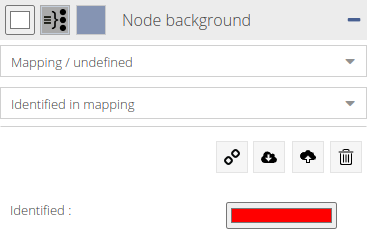
\includegraphics{images/metexplore_node_bg_mapped.png}

}

}

\end{minipage}%

\end{figure}

\begin{center}\rule{0.5\linewidth}{0.5pt}\end{center}

\hypertarget{input-metabolites-highlighted-in-red}{%
\subsubsection{Input metabolites highlighted in
red}\label{input-metabolites-highlighted-in-red}}

\begin{figure}

{\centering 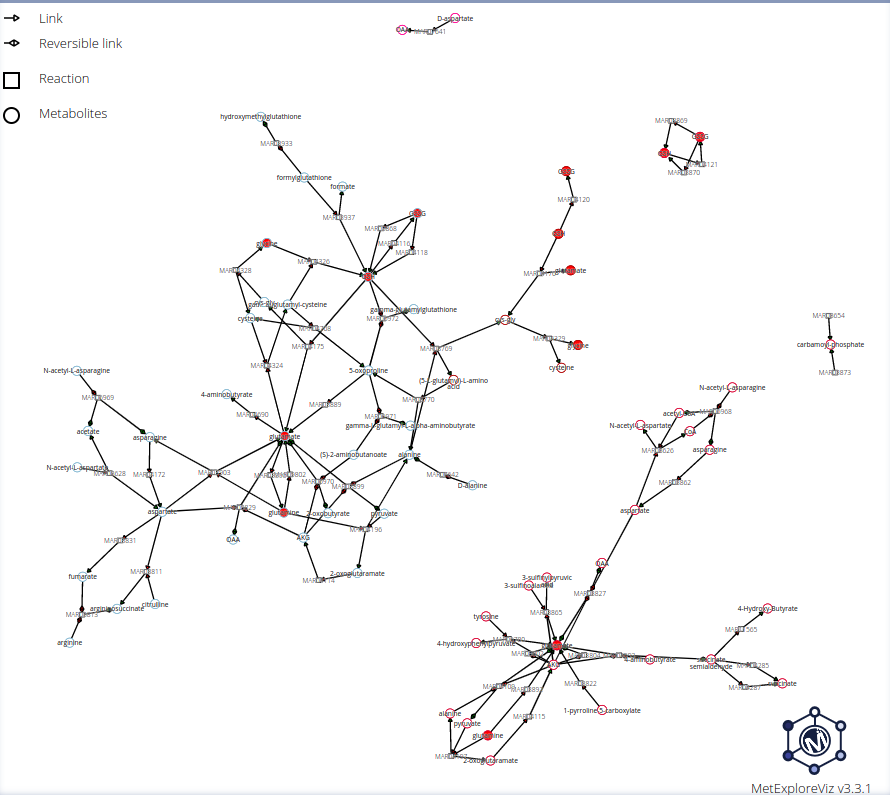
\includegraphics{images/metexplore_viz_node_bg.png}

}

\end{figure}

\begin{center}\rule{0.5\linewidth}{0.5pt}\end{center}

\hypertarget{changing-widthheight-and-roundness}{%
\subsubsection{Changing width/height and
roundness}\label{changing-widthheight-and-roundness}}

You can further enhance your visualisation by changing the width and
height of mapped metabolites in a similar fashion.

\begin{figure}

\begin{minipage}[t]{0.50\linewidth}

{\centering 

\raisebox{-\height}{

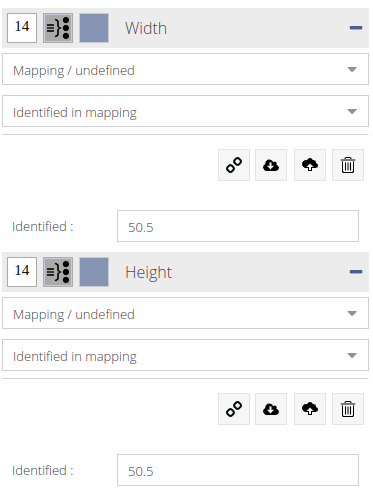
\includegraphics{images/metexplore_width_height.png}

}

}

\end{minipage}%
%
\begin{minipage}[t]{0.50\linewidth}

{\centering 

\raisebox{-\height}{

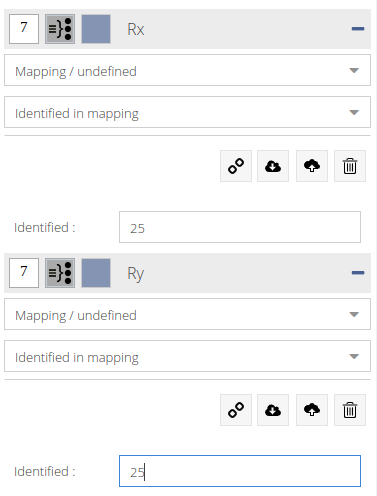
\includegraphics{images/metexplore_rx_ry.png}

}

}

\end{minipage}%

\end{figure}

\begin{center}\rule{0.5\linewidth}{0.5pt}\end{center}

\hypertarget{larger-nodes-for-input-metabolites}{%
\subsubsection{Larger nodes for input
metabolites}\label{larger-nodes-for-input-metabolites}}

\begin{figure}

{\centering 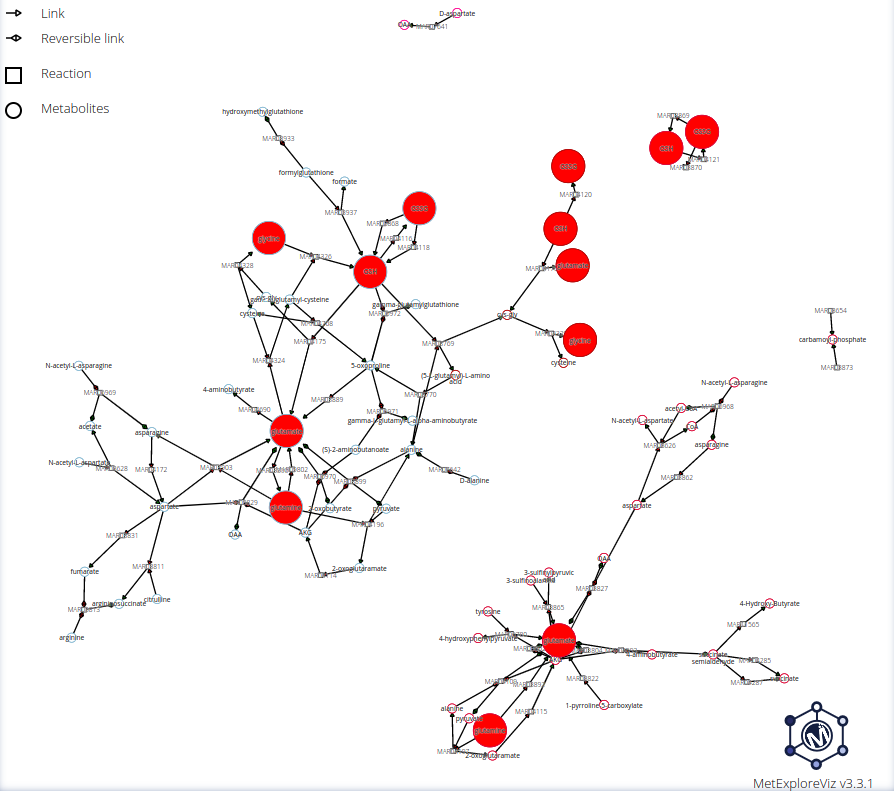
\includegraphics{images/metexplore_viz_large.png}

}

\end{figure}

\hypertarget{other-mapping}{%
\subsection{Other mapping}\label{other-mapping}}

Instead of mapping all of your metabolomics dataset, you could map the
leading edge metabolites from GSEA (which is a subset of your data for
one pathway).

You can visualise more than one pathway at once, but too many will be
very slow to load!



\end{document}
